\documentclass[twoside]{book}

% Packages required by doxygen
\usepackage{fixltx2e}
\usepackage{calc}
\usepackage{doxygen}
\usepackage[export]{adjustbox} % also loads graphicx
\usepackage{graphicx}
\usepackage[utf8]{inputenc}
\usepackage{makeidx}
\usepackage{multicol}
\usepackage{multirow}
\PassOptionsToPackage{warn}{textcomp}
\usepackage{textcomp}
\usepackage[nointegrals]{wasysym}
\usepackage[table]{xcolor}

% Font selection
\usepackage[T1]{fontenc}
\usepackage[scaled=.90]{helvet}
\usepackage{courier}
\usepackage{amssymb}
\usepackage{sectsty}
\renewcommand{\familydefault}{\sfdefault}
\allsectionsfont{%
  \fontseries{bc}\selectfont%
  \color{darkgray}%
}
\renewcommand{\DoxyLabelFont}{%
  \fontseries{bc}\selectfont%
  \color{darkgray}%
}
\newcommand{\+}{\discretionary{\mbox{\scriptsize$\hookleftarrow$}}{}{}}

% Page & text layout
\usepackage{geometry}
\geometry{%
  a4paper,%
  top=2.5cm,%
  bottom=2.5cm,%
  left=2.5cm,%
  right=2.5cm%
}
\tolerance=750
\hfuzz=15pt
\hbadness=750
\setlength{\emergencystretch}{15pt}
\setlength{\parindent}{0cm}
\setlength{\parskip}{3ex plus 2ex minus 2ex}
\makeatletter
\renewcommand{\paragraph}{%
  \@startsection{paragraph}{4}{0ex}{-1.0ex}{1.0ex}{%
    \normalfont\normalsize\bfseries\SS@parafont%
  }%
}
\renewcommand{\subparagraph}{%
  \@startsection{subparagraph}{5}{0ex}{-1.0ex}{1.0ex}{%
    \normalfont\normalsize\bfseries\SS@subparafont%
  }%
}
\makeatother

% Headers & footers
\usepackage{fancyhdr}
\pagestyle{fancyplain}
\fancyhead[LE]{\fancyplain{}{\bfseries\thepage}}
\fancyhead[CE]{\fancyplain{}{}}
\fancyhead[RE]{\fancyplain{}{\bfseries\leftmark}}
\fancyhead[LO]{\fancyplain{}{\bfseries\rightmark}}
\fancyhead[CO]{\fancyplain{}{}}
\fancyhead[RO]{\fancyplain{}{\bfseries\thepage}}
\fancyfoot[LE]{\fancyplain{}{}}
\fancyfoot[CE]{\fancyplain{}{}}
\fancyfoot[RE]{\fancyplain{}{\bfseries\scriptsize Generated by Doxygen }}
\fancyfoot[LO]{\fancyplain{}{\bfseries\scriptsize Generated by Doxygen }}
\fancyfoot[CO]{\fancyplain{}{}}
\fancyfoot[RO]{\fancyplain{}{}}
\renewcommand{\footrulewidth}{0.4pt}
\renewcommand{\chaptermark}[1]{%
  \markboth{#1}{}%
}
\renewcommand{\sectionmark}[1]{%
  \markright{\thesection\ #1}%
}

% Indices & bibliography
\usepackage{natbib}
\usepackage[titles]{tocloft}
\setcounter{tocdepth}{3}
\setcounter{secnumdepth}{5}
\makeindex

% Hyperlinks (required, but should be loaded last)
\usepackage{ifpdf}
\ifpdf
  \usepackage[pdftex,pagebackref=true]{hyperref}
\else
  \usepackage[ps2pdf,pagebackref=true]{hyperref}
\fi
\hypersetup{%
  colorlinks=true,%
  linkcolor=blue,%
  citecolor=blue,%
  unicode%
}

% Custom commands
\newcommand{\clearemptydoublepage}{%
  \newpage{\pagestyle{empty}\cleardoublepage}%
}

\usepackage{caption}
\captionsetup{labelsep=space,justification=centering,font={bf},singlelinecheck=off,skip=4pt,position=top}

%===== C O N T E N T S =====

\begin{document}

% Titlepage & ToC
\hypersetup{pageanchor=false,
             bookmarksnumbered=true,
             pdfencoding=unicode
            }
\pagenumbering{alph}
\begin{titlepage}
\vspace*{7cm}
\begin{center}%
{\Large Command and Data Handeling Test Assignment }\\
\vspace*{1cm}
{\large Generated by Doxygen 1.8.12}\\
\end{center}
\end{titlepage}
\clearemptydoublepage
\pagenumbering{roman}
\tableofcontents
\clearemptydoublepage
\pagenumbering{arabic}
\hypersetup{pageanchor=true}

%--- Begin generated contents ---
\chapter{R\+E\+A\+D\+ME}
\label{md_README}
\hypertarget{md_README}{}
The program creates a \hyperlink{classPowerTeam}{Power\+Team} object with a set power level it then charges a battery object with this power level. 
\chapter{Hierarchical Index}
\section{Class Hierarchy}
This inheritance list is sorted roughly, but not completely, alphabetically\+:\begin{DoxyCompactList}
\item \contentsline{section}{Battery}{\pageref{classBattery}}{}
\item Exception\begin{DoxyCompactList}
\item \contentsline{section}{cpplint.\+\_\+\+Include\+Error}{\pageref{classcpplint_1_1__IncludeError}}{}
\end{DoxyCompactList}
\item object\begin{DoxyCompactList}
\item \contentsline{section}{cpplint.\+\_\+\+Block\+Info}{\pageref{classcpplint_1_1__BlockInfo}}{}
\begin{DoxyCompactList}
\item \contentsline{section}{cpplint.\+\_\+\+Class\+Info}{\pageref{classcpplint_1_1__ClassInfo}}{}
\item \contentsline{section}{cpplint.\+\_\+\+Extern\+C\+Info}{\pageref{classcpplint_1_1__ExternCInfo}}{}
\item \contentsline{section}{cpplint.\+\_\+\+Namespace\+Info}{\pageref{classcpplint_1_1__NamespaceInfo}}{}
\end{DoxyCompactList}
\item \contentsline{section}{cpplint.\+\_\+\+Cpp\+Lint\+State}{\pageref{classcpplint_1_1__CppLintState}}{}
\item \contentsline{section}{cpplint.\+\_\+\+Function\+State}{\pageref{classcpplint_1_1__FunctionState}}{}
\item \contentsline{section}{cpplint.\+\_\+\+Include\+State}{\pageref{classcpplint_1_1__IncludeState}}{}
\item \contentsline{section}{cpplint.\+\_\+\+Preprocessor\+Info}{\pageref{classcpplint_1_1__PreprocessorInfo}}{}
\item \contentsline{section}{cpplint.\+Cleansed\+Lines}{\pageref{classcpplint_1_1CleansedLines}}{}
\item \contentsline{section}{cpplint.\+File\+Info}{\pageref{classcpplint_1_1FileInfo}}{}
\item \contentsline{section}{cpplint.\+Nesting\+State}{\pageref{classcpplint_1_1NestingState}}{}
\end{DoxyCompactList}
\item \contentsline{section}{Power\+Team}{\pageref{classPowerTeam}}{}
\end{DoxyCompactList}

\chapter{Class Index}
\section{Class List}
Here are the classes, structs, unions and interfaces with brief descriptions\+:\begin{DoxyCompactList}
\item\contentsline{section}{\hyperlink{classcpplint_1_1__BlockInfo}{cpplint.\+\_\+\+Block\+Info} }{\pageref{classcpplint_1_1__BlockInfo}}{}
\item\contentsline{section}{\hyperlink{classcpplint_1_1__ClassInfo}{cpplint.\+\_\+\+Class\+Info} }{\pageref{classcpplint_1_1__ClassInfo}}{}
\item\contentsline{section}{\hyperlink{classcpplint_1_1__CppLintState}{cpplint.\+\_\+\+Cpp\+Lint\+State} }{\pageref{classcpplint_1_1__CppLintState}}{}
\item\contentsline{section}{\hyperlink{classcpplint_1_1__ExternCInfo}{cpplint.\+\_\+\+Extern\+C\+Info} }{\pageref{classcpplint_1_1__ExternCInfo}}{}
\item\contentsline{section}{\hyperlink{classcpplint_1_1__FunctionState}{cpplint.\+\_\+\+Function\+State} }{\pageref{classcpplint_1_1__FunctionState}}{}
\item\contentsline{section}{\hyperlink{classcpplint_1_1__IncludeError}{cpplint.\+\_\+\+Include\+Error} }{\pageref{classcpplint_1_1__IncludeError}}{}
\item\contentsline{section}{\hyperlink{classcpplint_1_1__IncludeState}{cpplint.\+\_\+\+Include\+State} }{\pageref{classcpplint_1_1__IncludeState}}{}
\item\contentsline{section}{\hyperlink{classcpplint_1_1__NamespaceInfo}{cpplint.\+\_\+\+Namespace\+Info} }{\pageref{classcpplint_1_1__NamespaceInfo}}{}
\item\contentsline{section}{\hyperlink{classcpplint_1_1__PreprocessorInfo}{cpplint.\+\_\+\+Preprocessor\+Info} }{\pageref{classcpplint_1_1__PreprocessorInfo}}{}
\item\contentsline{section}{\hyperlink{classBattery}{Battery} }{\pageref{classBattery}}{}
\item\contentsline{section}{\hyperlink{classcpplint_1_1CleansedLines}{cpplint.\+Cleansed\+Lines} }{\pageref{classcpplint_1_1CleansedLines}}{}
\item\contentsline{section}{\hyperlink{classcpplint_1_1FileInfo}{cpplint.\+File\+Info} }{\pageref{classcpplint_1_1FileInfo}}{}
\item\contentsline{section}{\hyperlink{classcpplint_1_1NestingState}{cpplint.\+Nesting\+State} }{\pageref{classcpplint_1_1NestingState}}{}
\item\contentsline{section}{\hyperlink{classPowerTeam}{Power\+Team} }{\pageref{classPowerTeam}}{}
\end{DoxyCompactList}

\chapter{File Index}
\section{File List}
Here is a list of all documented files with brief descriptions\+:\begin{DoxyCompactList}
\item\contentsline{section}{\hyperlink{battery_8cpp}{battery.\+cpp} }{\pageref{battery_8cpp}}{}
\item\contentsline{section}{\hyperlink{battery_8h}{battery.\+h} }{\pageref{battery_8h}}{}
\item\contentsline{section}{\hyperlink{main_8cpp}{main.\+cpp} }{\pageref{main_8cpp}}{}
\item\contentsline{section}{\hyperlink{power_8cpp}{power.\+cpp} }{\pageref{power_8cpp}}{}
\item\contentsline{section}{\hyperlink{power_8h}{power.\+h} }{\pageref{power_8h}}{}
\end{DoxyCompactList}

\chapter{Class Documentation}
\hypertarget{classcpplint_1_1__BlockInfo}{}\section{cpplint.\+\_\+\+Block\+Info Class Reference}
\label{classcpplint_1_1__BlockInfo}\index{cpplint.\+\_\+\+Block\+Info@{cpplint.\+\_\+\+Block\+Info}}
Inheritance diagram for cpplint.\+\_\+\+Block\+Info\+:\begin{figure}[H]
\begin{center}
\leavevmode
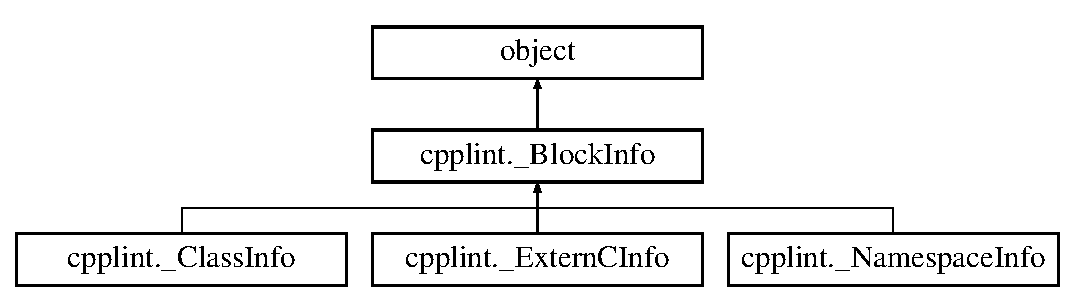
\includegraphics[height=3.000000cm]{classcpplint_1_1__BlockInfo}
\end{center}
\end{figure}
\subsection*{Public Member Functions}
\begin{DoxyCompactItemize}
\item 
def {\bfseries \+\_\+\+\_\+init\+\_\+\+\_\+} (self, seen\+\_\+open\+\_\+brace)\hypertarget{classcpplint_1_1__BlockInfo_aeb3be53b1a456b9ea4f7cc6e15b4b14e}{}\label{classcpplint_1_1__BlockInfo_aeb3be53b1a456b9ea4f7cc6e15b4b14e}

\item 
def \hyperlink{classcpplint_1_1__BlockInfo_af316a9e3623b45bd07079166be67582c}{Check\+Begin} (self, filename, clean\+\_\+lines, linenum, error)
\item 
def \hyperlink{classcpplint_1_1__BlockInfo_ae504a3429de136eebf85f32fcae6a8ca}{Check\+End} (self, filename, clean\+\_\+lines, linenum, error)
\item 
def \hyperlink{classcpplint_1_1__BlockInfo_ab3e06a94a38d7397ce6a4faa094010d4}{Is\+Block\+Info} (self)
\end{DoxyCompactItemize}
\subsection*{Public Attributes}
\begin{DoxyCompactItemize}
\item 
{\bfseries seen\+\_\+open\+\_\+brace}\hypertarget{classcpplint_1_1__BlockInfo_aa974539217437751383ad20896c974d7}{}\label{classcpplint_1_1__BlockInfo_aa974539217437751383ad20896c974d7}

\item 
{\bfseries open\+\_\+parentheses}\hypertarget{classcpplint_1_1__BlockInfo_a02a0b48995a599f6b2bbaa6f16cca98a}{}\label{classcpplint_1_1__BlockInfo_a02a0b48995a599f6b2bbaa6f16cca98a}

\item 
{\bfseries inline\+\_\+asm}\hypertarget{classcpplint_1_1__BlockInfo_aad762ef7088f2f556a75c9a80006f4db}{}\label{classcpplint_1_1__BlockInfo_aad762ef7088f2f556a75c9a80006f4db}

\item 
{\bfseries check\+\_\+namespace\+\_\+indentation}\hypertarget{classcpplint_1_1__BlockInfo_a120822b07db37b3480a573ec29ee4457}{}\label{classcpplint_1_1__BlockInfo_a120822b07db37b3480a573ec29ee4457}

\end{DoxyCompactItemize}


\subsection{Detailed Description}
\begin{DoxyVerb}Stores information about a generic block of code.\end{DoxyVerb}
 

\subsection{Member Function Documentation}
\index{cpplint\+::\+\_\+\+Block\+Info@{cpplint\+::\+\_\+\+Block\+Info}!Check\+Begin@{Check\+Begin}}
\index{Check\+Begin@{Check\+Begin}!cpplint\+::\+\_\+\+Block\+Info@{cpplint\+::\+\_\+\+Block\+Info}}
\subsubsection[{\texorpdfstring{Check\+Begin(self, filename, clean\+\_\+lines, linenum, error)}{CheckBegin(self, filename, clean\_lines, linenum, error)}}]{\setlength{\rightskip}{0pt plus 5cm}def cpplint.\+\_\+\+Block\+Info.\+Check\+Begin (
\begin{DoxyParamCaption}
\item[{}]{self, }
\item[{}]{filename, }
\item[{}]{clean\+\_\+lines, }
\item[{}]{linenum, }
\item[{}]{error}
\end{DoxyParamCaption}
)}\hypertarget{classcpplint_1_1__BlockInfo_af316a9e3623b45bd07079166be67582c}{}\label{classcpplint_1_1__BlockInfo_af316a9e3623b45bd07079166be67582c}
\begin{DoxyVerb}Run checks that applies to text up to the opening brace.

This is mostly for checking the text after the class identifier
and the "{", usually where the base class is specified.  For other
blocks, there isn't much to check, so we always pass.

Args:
  filename: The name of the current file.
  clean_lines: A CleansedLines instance containing the file.
  linenum: The number of the line to check.
  error: The function to call with any errors found.
\end{DoxyVerb}
 \index{cpplint\+::\+\_\+\+Block\+Info@{cpplint\+::\+\_\+\+Block\+Info}!Check\+End@{Check\+End}}
\index{Check\+End@{Check\+End}!cpplint\+::\+\_\+\+Block\+Info@{cpplint\+::\+\_\+\+Block\+Info}}
\subsubsection[{\texorpdfstring{Check\+End(self, filename, clean\+\_\+lines, linenum, error)}{CheckEnd(self, filename, clean\_lines, linenum, error)}}]{\setlength{\rightskip}{0pt plus 5cm}def cpplint.\+\_\+\+Block\+Info.\+Check\+End (
\begin{DoxyParamCaption}
\item[{}]{self, }
\item[{}]{filename, }
\item[{}]{clean\+\_\+lines, }
\item[{}]{linenum, }
\item[{}]{error}
\end{DoxyParamCaption}
)}\hypertarget{classcpplint_1_1__BlockInfo_ae504a3429de136eebf85f32fcae6a8ca}{}\label{classcpplint_1_1__BlockInfo_ae504a3429de136eebf85f32fcae6a8ca}
\begin{DoxyVerb}Run checks that applies to text after the closing brace.

This is mostly used for checking end of namespace comments.

Args:
  filename: The name of the current file.
  clean_lines: A CleansedLines instance containing the file.
  linenum: The number of the line to check.
  error: The function to call with any errors found.
\end{DoxyVerb}
 \index{cpplint\+::\+\_\+\+Block\+Info@{cpplint\+::\+\_\+\+Block\+Info}!Is\+Block\+Info@{Is\+Block\+Info}}
\index{Is\+Block\+Info@{Is\+Block\+Info}!cpplint\+::\+\_\+\+Block\+Info@{cpplint\+::\+\_\+\+Block\+Info}}
\subsubsection[{\texorpdfstring{Is\+Block\+Info(self)}{IsBlockInfo(self)}}]{\setlength{\rightskip}{0pt plus 5cm}def cpplint.\+\_\+\+Block\+Info.\+Is\+Block\+Info (
\begin{DoxyParamCaption}
\item[{}]{self}
\end{DoxyParamCaption}
)}\hypertarget{classcpplint_1_1__BlockInfo_ab3e06a94a38d7397ce6a4faa094010d4}{}\label{classcpplint_1_1__BlockInfo_ab3e06a94a38d7397ce6a4faa094010d4}
\begin{DoxyVerb}Returns true if this block is a _BlockInfo.

This is convenient for verifying that an object is an instance of
a _BlockInfo, but not an instance of any of the derived classes.

Returns:
  True for this class, False for derived classes.
\end{DoxyVerb}
 

The documentation for this class was generated from the following file\+:\begin{DoxyCompactItemize}
\item 
cpplint.\+py\end{DoxyCompactItemize}

\hypertarget{classcpplint_1_1__ClassInfo}{}\section{cpplint.\+\_\+\+Class\+Info Class Reference}
\label{classcpplint_1_1__ClassInfo}\index{cpplint.\+\_\+\+Class\+Info@{cpplint.\+\_\+\+Class\+Info}}
Inheritance diagram for cpplint.\+\_\+\+Class\+Info\+:\begin{figure}[H]
\begin{center}
\leavevmode
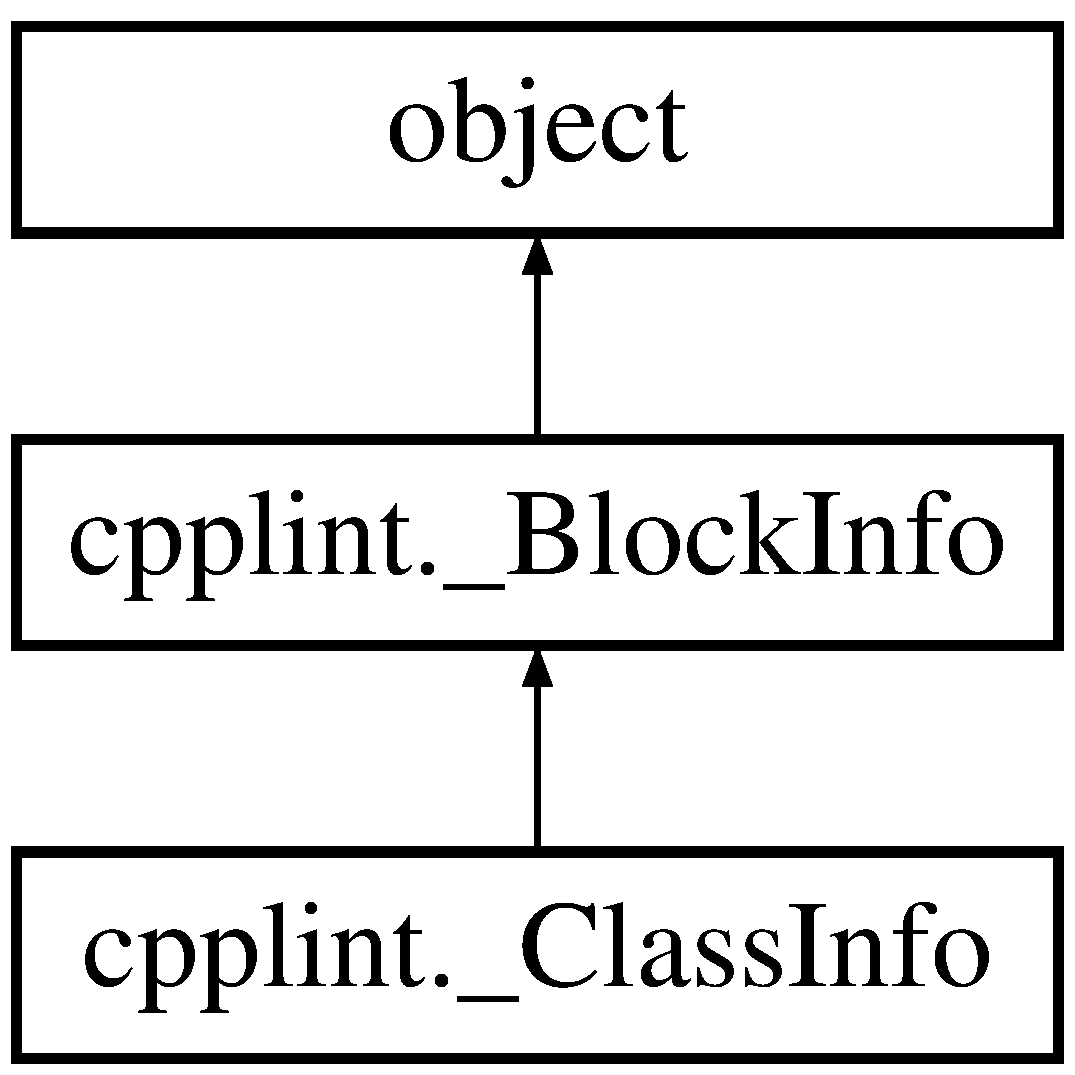
\includegraphics[height=3.000000cm]{classcpplint_1_1__ClassInfo}
\end{center}
\end{figure}
\subsection*{Public Member Functions}
\begin{DoxyCompactItemize}
\item 
def {\bfseries \+\_\+\+\_\+init\+\_\+\+\_\+} (self, name, class\+\_\+or\+\_\+struct, clean\+\_\+lines, linenum)\hypertarget{classcpplint_1_1__ClassInfo_a549b13e77acbe712f79a2d2b2c98ff7d}{}\label{classcpplint_1_1__ClassInfo_a549b13e77acbe712f79a2d2b2c98ff7d}

\item 
def {\bfseries Check\+Begin} (self, filename, clean\+\_\+lines, linenum, error)\hypertarget{classcpplint_1_1__ClassInfo_abed47237f2e7416ca51cb220cfad6c1b}{}\label{classcpplint_1_1__ClassInfo_abed47237f2e7416ca51cb220cfad6c1b}

\item 
def {\bfseries Check\+End} (self, filename, clean\+\_\+lines, linenum, error)\hypertarget{classcpplint_1_1__ClassInfo_a8a61461a72928bc6ce62a9b75b770fec}{}\label{classcpplint_1_1__ClassInfo_a8a61461a72928bc6ce62a9b75b770fec}

\end{DoxyCompactItemize}
\subsection*{Public Attributes}
\begin{DoxyCompactItemize}
\item 
{\bfseries name}\hypertarget{classcpplint_1_1__ClassInfo_a3de5f207d3449d735d15ebca779fe336}{}\label{classcpplint_1_1__ClassInfo_a3de5f207d3449d735d15ebca779fe336}

\item 
{\bfseries starting\+\_\+linenum}\hypertarget{classcpplint_1_1__ClassInfo_a0c8df96999cd0c160fbb9e3c1ca0ac55}{}\label{classcpplint_1_1__ClassInfo_a0c8df96999cd0c160fbb9e3c1ca0ac55}

\item 
{\bfseries is\+\_\+derived}\hypertarget{classcpplint_1_1__ClassInfo_a8cace481686fbbb35a1da552646aa9f4}{}\label{classcpplint_1_1__ClassInfo_a8cace481686fbbb35a1da552646aa9f4}

\item 
{\bfseries check\+\_\+namespace\+\_\+indentation}\hypertarget{classcpplint_1_1__ClassInfo_a0ead95c17ac0b293d0d371eb7b414bd9}{}\label{classcpplint_1_1__ClassInfo_a0ead95c17ac0b293d0d371eb7b414bd9}

\item 
{\bfseries access}\hypertarget{classcpplint_1_1__ClassInfo_aef1251c699b50c6603ce38ca8cce414c}{}\label{classcpplint_1_1__ClassInfo_aef1251c699b50c6603ce38ca8cce414c}

\item 
{\bfseries is\+\_\+struct}\hypertarget{classcpplint_1_1__ClassInfo_a57b443f42838d73183921d661b6fe4ef}{}\label{classcpplint_1_1__ClassInfo_a57b443f42838d73183921d661b6fe4ef}

\item 
{\bfseries class\+\_\+indent}\hypertarget{classcpplint_1_1__ClassInfo_adc7d328734cc58fe46a3a3f323a09f4a}{}\label{classcpplint_1_1__ClassInfo_adc7d328734cc58fe46a3a3f323a09f4a}

\item 
{\bfseries last\+\_\+line}\hypertarget{classcpplint_1_1__ClassInfo_a72e0f4576cdcb6f3886ed52e2affbc75}{}\label{classcpplint_1_1__ClassInfo_a72e0f4576cdcb6f3886ed52e2affbc75}

\end{DoxyCompactItemize}


\subsection{Detailed Description}
\begin{DoxyVerb}Stores information about a class.\end{DoxyVerb}
 

The documentation for this class was generated from the following file\+:\begin{DoxyCompactItemize}
\item 
cpplint.\+py\end{DoxyCompactItemize}

\hypertarget{classcpplint_1_1__CppLintState}{}\section{cpplint.\+\_\+\+Cpp\+Lint\+State Class Reference}
\label{classcpplint_1_1__CppLintState}\index{cpplint.\+\_\+\+Cpp\+Lint\+State@{cpplint.\+\_\+\+Cpp\+Lint\+State}}
Inheritance diagram for cpplint.\+\_\+\+Cpp\+Lint\+State\+:\begin{figure}[H]
\begin{center}
\leavevmode
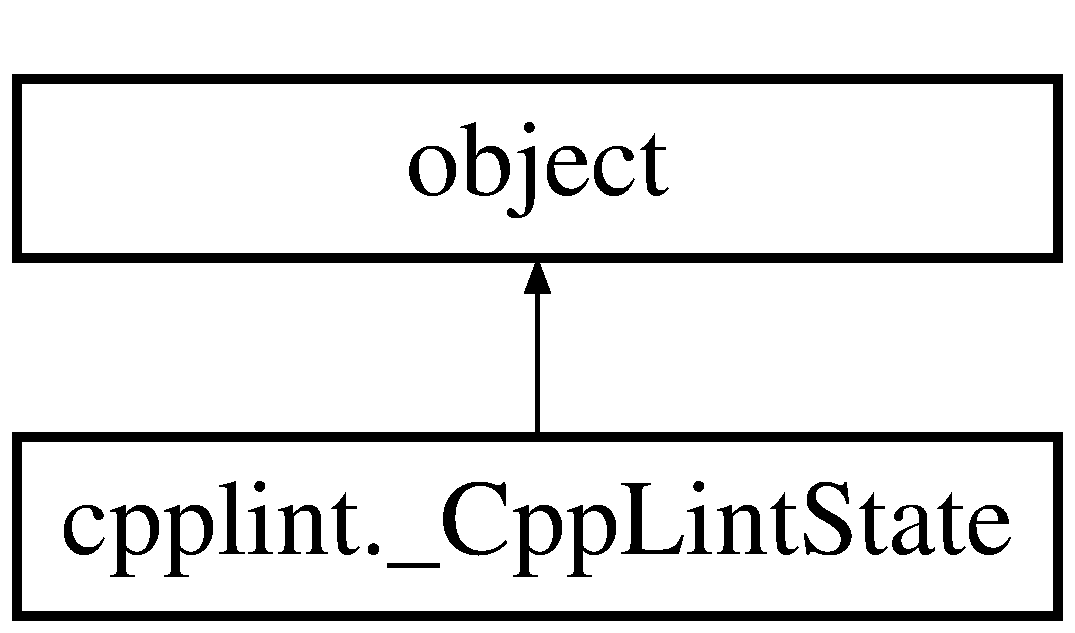
\includegraphics[height=2.000000cm]{classcpplint_1_1__CppLintState}
\end{center}
\end{figure}
\subsection*{Public Member Functions}
\begin{DoxyCompactItemize}
\item 
def {\bfseries \+\_\+\+\_\+init\+\_\+\+\_\+} (self)\hypertarget{classcpplint_1_1__CppLintState_a9cc2db6b8d2e3b757fc48fb3c2fd4d8b}{}\label{classcpplint_1_1__CppLintState_a9cc2db6b8d2e3b757fc48fb3c2fd4d8b}

\item 
def \hyperlink{classcpplint_1_1__CppLintState_ab43553d2e2027b58d08a7001c71c0902}{Set\+Output\+Format} (self, output\+\_\+format)
\item 
def \hyperlink{classcpplint_1_1__CppLintState_ad4f97c907cc79e8d60237d0327830588}{Set\+Verbose\+Level} (self, level)
\item 
def \hyperlink{classcpplint_1_1__CppLintState_ac2503f2d8a357edd3ca648d219c7317e}{Set\+Counting\+Style} (self, counting\+\_\+style)
\item 
def \hyperlink{classcpplint_1_1__CppLintState_a359d4516eac0c1dce6223cf18181ac80}{Set\+Filters} (self, filters)
\item 
def \hyperlink{classcpplint_1_1__CppLintState_a248c70895572f2468d3c842faff2f285}{Add\+Filters} (self, filters)
\item 
def \hyperlink{classcpplint_1_1__CppLintState_a2444e784910e03681de22f43d4077dd1}{Backup\+Filters} (self)
\item 
def \hyperlink{classcpplint_1_1__CppLintState_a7a9c9fdfe033ebe1933450b4ae524598}{Restore\+Filters} (self)
\item 
def \hyperlink{classcpplint_1_1__CppLintState_ab802596abd5fba5e290e090388b6842a}{Reset\+Error\+Counts} (self)
\item 
def \hyperlink{classcpplint_1_1__CppLintState_a27a33a5049850d52cc8aef3478ca445a}{Increment\+Error\+Count} (self, category)
\item 
def \hyperlink{classcpplint_1_1__CppLintState_a3149156b00f8d53e5625256e3df2b4f0}{Print\+Error\+Counts} (self)
\end{DoxyCompactItemize}
\subsection*{Public Attributes}
\begin{DoxyCompactItemize}
\item 
{\bfseries verbose\+\_\+level}\hypertarget{classcpplint_1_1__CppLintState_a94328754c2f7481f4da9757a9dede308}{}\label{classcpplint_1_1__CppLintState_a94328754c2f7481f4da9757a9dede308}

\item 
{\bfseries error\+\_\+count}\hypertarget{classcpplint_1_1__CppLintState_a4039ff9668057eff4549b99905ce753b}{}\label{classcpplint_1_1__CppLintState_a4039ff9668057eff4549b99905ce753b}

\item 
{\bfseries filters}\hypertarget{classcpplint_1_1__CppLintState_a8443105b9623383ab75fa242009c006e}{}\label{classcpplint_1_1__CppLintState_a8443105b9623383ab75fa242009c006e}

\item 
{\bfseries counting}\hypertarget{classcpplint_1_1__CppLintState_acd4f4157637d141a4de63bf10d2ca755}{}\label{classcpplint_1_1__CppLintState_acd4f4157637d141a4de63bf10d2ca755}

\item 
{\bfseries errors\+\_\+by\+\_\+category}\hypertarget{classcpplint_1_1__CppLintState_afb33527113706b5fcae07d680d8cec99}{}\label{classcpplint_1_1__CppLintState_afb33527113706b5fcae07d680d8cec99}

\item 
{\bfseries output\+\_\+format}\hypertarget{classcpplint_1_1__CppLintState_a5c68ca79b0ff9b2fba1c488a7b2bd3f0}{}\label{classcpplint_1_1__CppLintState_a5c68ca79b0ff9b2fba1c488a7b2bd3f0}

\end{DoxyCompactItemize}


\subsection{Detailed Description}
\begin{DoxyVerb}Maintains module-wide state..\end{DoxyVerb}
 

\subsection{Member Function Documentation}
\index{cpplint\+::\+\_\+\+Cpp\+Lint\+State@{cpplint\+::\+\_\+\+Cpp\+Lint\+State}!Add\+Filters@{Add\+Filters}}
\index{Add\+Filters@{Add\+Filters}!cpplint\+::\+\_\+\+Cpp\+Lint\+State@{cpplint\+::\+\_\+\+Cpp\+Lint\+State}}
\subsubsection[{\texorpdfstring{Add\+Filters(self, filters)}{AddFilters(self, filters)}}]{\setlength{\rightskip}{0pt plus 5cm}def cpplint.\+\_\+\+Cpp\+Lint\+State.\+Add\+Filters (
\begin{DoxyParamCaption}
\item[{}]{self, }
\item[{}]{filters}
\end{DoxyParamCaption}
)}\hypertarget{classcpplint_1_1__CppLintState_a248c70895572f2468d3c842faff2f285}{}\label{classcpplint_1_1__CppLintState_a248c70895572f2468d3c842faff2f285}
\begin{DoxyVerb}Adds more filters to the existing list of error-message filters. \end{DoxyVerb}
 \index{cpplint\+::\+\_\+\+Cpp\+Lint\+State@{cpplint\+::\+\_\+\+Cpp\+Lint\+State}!Backup\+Filters@{Backup\+Filters}}
\index{Backup\+Filters@{Backup\+Filters}!cpplint\+::\+\_\+\+Cpp\+Lint\+State@{cpplint\+::\+\_\+\+Cpp\+Lint\+State}}
\subsubsection[{\texorpdfstring{Backup\+Filters(self)}{BackupFilters(self)}}]{\setlength{\rightskip}{0pt plus 5cm}def cpplint.\+\_\+\+Cpp\+Lint\+State.\+Backup\+Filters (
\begin{DoxyParamCaption}
\item[{}]{self}
\end{DoxyParamCaption}
)}\hypertarget{classcpplint_1_1__CppLintState_a2444e784910e03681de22f43d4077dd1}{}\label{classcpplint_1_1__CppLintState_a2444e784910e03681de22f43d4077dd1}
\begin{DoxyVerb}Saves the current filter list to backup storage.\end{DoxyVerb}
 \index{cpplint\+::\+\_\+\+Cpp\+Lint\+State@{cpplint\+::\+\_\+\+Cpp\+Lint\+State}!Increment\+Error\+Count@{Increment\+Error\+Count}}
\index{Increment\+Error\+Count@{Increment\+Error\+Count}!cpplint\+::\+\_\+\+Cpp\+Lint\+State@{cpplint\+::\+\_\+\+Cpp\+Lint\+State}}
\subsubsection[{\texorpdfstring{Increment\+Error\+Count(self, category)}{IncrementErrorCount(self, category)}}]{\setlength{\rightskip}{0pt plus 5cm}def cpplint.\+\_\+\+Cpp\+Lint\+State.\+Increment\+Error\+Count (
\begin{DoxyParamCaption}
\item[{}]{self, }
\item[{}]{category}
\end{DoxyParamCaption}
)}\hypertarget{classcpplint_1_1__CppLintState_a27a33a5049850d52cc8aef3478ca445a}{}\label{classcpplint_1_1__CppLintState_a27a33a5049850d52cc8aef3478ca445a}
\begin{DoxyVerb}Bumps the module's error statistic.\end{DoxyVerb}
 \index{cpplint\+::\+\_\+\+Cpp\+Lint\+State@{cpplint\+::\+\_\+\+Cpp\+Lint\+State}!Print\+Error\+Counts@{Print\+Error\+Counts}}
\index{Print\+Error\+Counts@{Print\+Error\+Counts}!cpplint\+::\+\_\+\+Cpp\+Lint\+State@{cpplint\+::\+\_\+\+Cpp\+Lint\+State}}
\subsubsection[{\texorpdfstring{Print\+Error\+Counts(self)}{PrintErrorCounts(self)}}]{\setlength{\rightskip}{0pt plus 5cm}def cpplint.\+\_\+\+Cpp\+Lint\+State.\+Print\+Error\+Counts (
\begin{DoxyParamCaption}
\item[{}]{self}
\end{DoxyParamCaption}
)}\hypertarget{classcpplint_1_1__CppLintState_a3149156b00f8d53e5625256e3df2b4f0}{}\label{classcpplint_1_1__CppLintState_a3149156b00f8d53e5625256e3df2b4f0}
\begin{DoxyVerb}Print a summary of errors by category, and the total.\end{DoxyVerb}
 \index{cpplint\+::\+\_\+\+Cpp\+Lint\+State@{cpplint\+::\+\_\+\+Cpp\+Lint\+State}!Reset\+Error\+Counts@{Reset\+Error\+Counts}}
\index{Reset\+Error\+Counts@{Reset\+Error\+Counts}!cpplint\+::\+\_\+\+Cpp\+Lint\+State@{cpplint\+::\+\_\+\+Cpp\+Lint\+State}}
\subsubsection[{\texorpdfstring{Reset\+Error\+Counts(self)}{ResetErrorCounts(self)}}]{\setlength{\rightskip}{0pt plus 5cm}def cpplint.\+\_\+\+Cpp\+Lint\+State.\+Reset\+Error\+Counts (
\begin{DoxyParamCaption}
\item[{}]{self}
\end{DoxyParamCaption}
)}\hypertarget{classcpplint_1_1__CppLintState_ab802596abd5fba5e290e090388b6842a}{}\label{classcpplint_1_1__CppLintState_ab802596abd5fba5e290e090388b6842a}
\begin{DoxyVerb}Sets the module's error statistic back to zero.\end{DoxyVerb}
 \index{cpplint\+::\+\_\+\+Cpp\+Lint\+State@{cpplint\+::\+\_\+\+Cpp\+Lint\+State}!Restore\+Filters@{Restore\+Filters}}
\index{Restore\+Filters@{Restore\+Filters}!cpplint\+::\+\_\+\+Cpp\+Lint\+State@{cpplint\+::\+\_\+\+Cpp\+Lint\+State}}
\subsubsection[{\texorpdfstring{Restore\+Filters(self)}{RestoreFilters(self)}}]{\setlength{\rightskip}{0pt plus 5cm}def cpplint.\+\_\+\+Cpp\+Lint\+State.\+Restore\+Filters (
\begin{DoxyParamCaption}
\item[{}]{self}
\end{DoxyParamCaption}
)}\hypertarget{classcpplint_1_1__CppLintState_a7a9c9fdfe033ebe1933450b4ae524598}{}\label{classcpplint_1_1__CppLintState_a7a9c9fdfe033ebe1933450b4ae524598}
\begin{DoxyVerb}Restores filters previously backed up.\end{DoxyVerb}
 \index{cpplint\+::\+\_\+\+Cpp\+Lint\+State@{cpplint\+::\+\_\+\+Cpp\+Lint\+State}!Set\+Counting\+Style@{Set\+Counting\+Style}}
\index{Set\+Counting\+Style@{Set\+Counting\+Style}!cpplint\+::\+\_\+\+Cpp\+Lint\+State@{cpplint\+::\+\_\+\+Cpp\+Lint\+State}}
\subsubsection[{\texorpdfstring{Set\+Counting\+Style(self, counting\+\_\+style)}{SetCountingStyle(self, counting\_style)}}]{\setlength{\rightskip}{0pt plus 5cm}def cpplint.\+\_\+\+Cpp\+Lint\+State.\+Set\+Counting\+Style (
\begin{DoxyParamCaption}
\item[{}]{self, }
\item[{}]{counting\+\_\+style}
\end{DoxyParamCaption}
)}\hypertarget{classcpplint_1_1__CppLintState_ac2503f2d8a357edd3ca648d219c7317e}{}\label{classcpplint_1_1__CppLintState_ac2503f2d8a357edd3ca648d219c7317e}
\begin{DoxyVerb}Sets the module's counting options.\end{DoxyVerb}
 \index{cpplint\+::\+\_\+\+Cpp\+Lint\+State@{cpplint\+::\+\_\+\+Cpp\+Lint\+State}!Set\+Filters@{Set\+Filters}}
\index{Set\+Filters@{Set\+Filters}!cpplint\+::\+\_\+\+Cpp\+Lint\+State@{cpplint\+::\+\_\+\+Cpp\+Lint\+State}}
\subsubsection[{\texorpdfstring{Set\+Filters(self, filters)}{SetFilters(self, filters)}}]{\setlength{\rightskip}{0pt plus 5cm}def cpplint.\+\_\+\+Cpp\+Lint\+State.\+Set\+Filters (
\begin{DoxyParamCaption}
\item[{}]{self, }
\item[{}]{filters}
\end{DoxyParamCaption}
)}\hypertarget{classcpplint_1_1__CppLintState_a359d4516eac0c1dce6223cf18181ac80}{}\label{classcpplint_1_1__CppLintState_a359d4516eac0c1dce6223cf18181ac80}
\begin{DoxyVerb}Sets the error-message filters.

These filters are applied when deciding whether to emit a given
error message.

Args:
  filters: A string of comma-separated filters (eg "+whitespace/indent").
       Each filter should start with + or -; else we die.

Raises:
  ValueError: The comma-separated filters did not all start with '+' or '-'.
          E.g. "-,+whitespace,-whitespace/indent,whitespace/badfilter"
\end{DoxyVerb}
 \index{cpplint\+::\+\_\+\+Cpp\+Lint\+State@{cpplint\+::\+\_\+\+Cpp\+Lint\+State}!Set\+Output\+Format@{Set\+Output\+Format}}
\index{Set\+Output\+Format@{Set\+Output\+Format}!cpplint\+::\+\_\+\+Cpp\+Lint\+State@{cpplint\+::\+\_\+\+Cpp\+Lint\+State}}
\subsubsection[{\texorpdfstring{Set\+Output\+Format(self, output\+\_\+format)}{SetOutputFormat(self, output\_format)}}]{\setlength{\rightskip}{0pt plus 5cm}def cpplint.\+\_\+\+Cpp\+Lint\+State.\+Set\+Output\+Format (
\begin{DoxyParamCaption}
\item[{}]{self, }
\item[{}]{output\+\_\+format}
\end{DoxyParamCaption}
)}\hypertarget{classcpplint_1_1__CppLintState_ab43553d2e2027b58d08a7001c71c0902}{}\label{classcpplint_1_1__CppLintState_ab43553d2e2027b58d08a7001c71c0902}
\begin{DoxyVerb}Sets the output format for errors.\end{DoxyVerb}
 \index{cpplint\+::\+\_\+\+Cpp\+Lint\+State@{cpplint\+::\+\_\+\+Cpp\+Lint\+State}!Set\+Verbose\+Level@{Set\+Verbose\+Level}}
\index{Set\+Verbose\+Level@{Set\+Verbose\+Level}!cpplint\+::\+\_\+\+Cpp\+Lint\+State@{cpplint\+::\+\_\+\+Cpp\+Lint\+State}}
\subsubsection[{\texorpdfstring{Set\+Verbose\+Level(self, level)}{SetVerboseLevel(self, level)}}]{\setlength{\rightskip}{0pt plus 5cm}def cpplint.\+\_\+\+Cpp\+Lint\+State.\+Set\+Verbose\+Level (
\begin{DoxyParamCaption}
\item[{}]{self, }
\item[{}]{level}
\end{DoxyParamCaption}
)}\hypertarget{classcpplint_1_1__CppLintState_ad4f97c907cc79e8d60237d0327830588}{}\label{classcpplint_1_1__CppLintState_ad4f97c907cc79e8d60237d0327830588}
\begin{DoxyVerb}Sets the module's verbosity, and returns the previous setting.\end{DoxyVerb}
 

The documentation for this class was generated from the following file\+:\begin{DoxyCompactItemize}
\item 
cpplint.\+py\end{DoxyCompactItemize}

\hypertarget{classcpplint_1_1__ExternCInfo}{}\section{cpplint.\+\_\+\+Extern\+C\+Info Class Reference}
\label{classcpplint_1_1__ExternCInfo}\index{cpplint.\+\_\+\+Extern\+C\+Info@{cpplint.\+\_\+\+Extern\+C\+Info}}
Inheritance diagram for cpplint.\+\_\+\+Extern\+C\+Info\+:\begin{figure}[H]
\begin{center}
\leavevmode
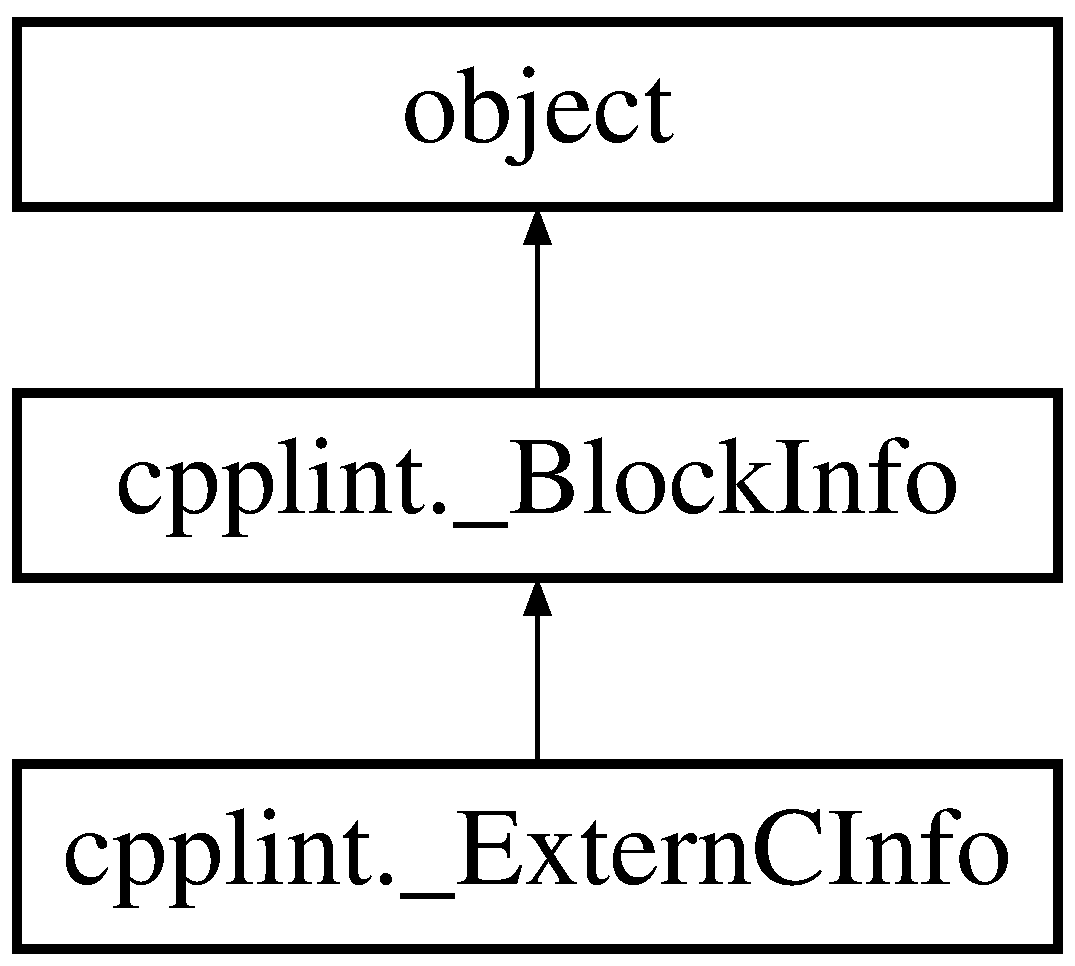
\includegraphics[height=3.000000cm]{classcpplint_1_1__ExternCInfo}
\end{center}
\end{figure}
\subsection*{Public Member Functions}
\begin{DoxyCompactItemize}
\item 
def {\bfseries \+\_\+\+\_\+init\+\_\+\+\_\+} (self)\hypertarget{classcpplint_1_1__ExternCInfo_a104a3dbf48a9fda7426775041d82f60a}{}\label{classcpplint_1_1__ExternCInfo_a104a3dbf48a9fda7426775041d82f60a}

\end{DoxyCompactItemize}
\subsection*{Additional Inherited Members}


\subsection{Detailed Description}
\begin{DoxyVerb}Stores information about an 'extern "C"' block.\end{DoxyVerb}
 

The documentation for this class was generated from the following file\+:\begin{DoxyCompactItemize}
\item 
cpplint.\+py\end{DoxyCompactItemize}

\hypertarget{classcpplint_1_1__FunctionState}{}\section{cpplint.\+\_\+\+Function\+State Class Reference}
\label{classcpplint_1_1__FunctionState}\index{cpplint.\+\_\+\+Function\+State@{cpplint.\+\_\+\+Function\+State}}
Inheritance diagram for cpplint.\+\_\+\+Function\+State\+:\begin{figure}[H]
\begin{center}
\leavevmode
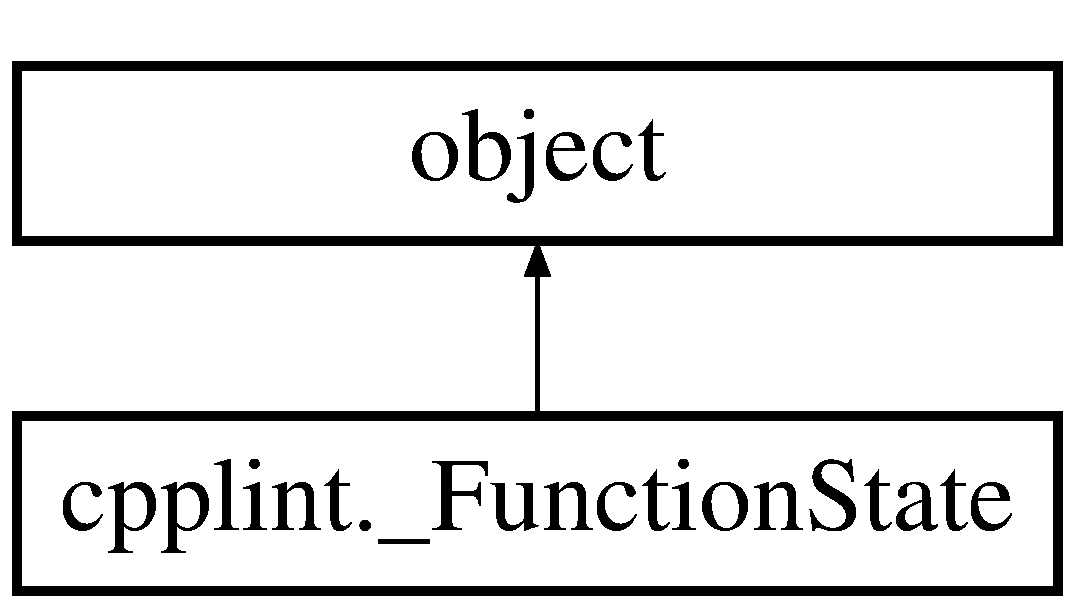
\includegraphics[height=2.000000cm]{classcpplint_1_1__FunctionState}
\end{center}
\end{figure}
\subsection*{Public Member Functions}
\begin{DoxyCompactItemize}
\item 
def {\bfseries \+\_\+\+\_\+init\+\_\+\+\_\+} (self)\hypertarget{classcpplint_1_1__FunctionState_a3f6a865710852cc74c6a7085180458ae}{}\label{classcpplint_1_1__FunctionState_a3f6a865710852cc74c6a7085180458ae}

\item 
def \hyperlink{classcpplint_1_1__FunctionState_a41215c4d73baccbb340f6d0df1c1f4b3}{Begin} (self, function\+\_\+name)
\item 
def \hyperlink{classcpplint_1_1__FunctionState_ac25c9711911ae181b091b52619cf2701}{Count} (self)
\item 
def \hyperlink{classcpplint_1_1__FunctionState_a5e4ad7d7b104038b45204ab4abf527b2}{Check} (self, error, filename, linenum)
\item 
def \hyperlink{classcpplint_1_1__FunctionState_a1ab6b0a575c25c135f9004b7fb12dc4a}{End} (self)
\end{DoxyCompactItemize}
\subsection*{Public Attributes}
\begin{DoxyCompactItemize}
\item 
{\bfseries in\+\_\+a\+\_\+function}\hypertarget{classcpplint_1_1__FunctionState_a8362d472591f60462184bf68b49c0efb}{}\label{classcpplint_1_1__FunctionState_a8362d472591f60462184bf68b49c0efb}

\item 
{\bfseries lines\+\_\+in\+\_\+function}\hypertarget{classcpplint_1_1__FunctionState_a886f5d476adc81f499a711750a399aa2}{}\label{classcpplint_1_1__FunctionState_a886f5d476adc81f499a711750a399aa2}

\item 
{\bfseries current\+\_\+function}\hypertarget{classcpplint_1_1__FunctionState_a320674f54bd75087febc8f0d83620569}{}\label{classcpplint_1_1__FunctionState_a320674f54bd75087febc8f0d83620569}

\end{DoxyCompactItemize}


\subsection{Detailed Description}
\begin{DoxyVerb}Tracks current function name and the number of lines in its body.\end{DoxyVerb}
 

\subsection{Member Function Documentation}
\index{cpplint\+::\+\_\+\+Function\+State@{cpplint\+::\+\_\+\+Function\+State}!Begin@{Begin}}
\index{Begin@{Begin}!cpplint\+::\+\_\+\+Function\+State@{cpplint\+::\+\_\+\+Function\+State}}
\subsubsection[{\texorpdfstring{Begin(self, function\+\_\+name)}{Begin(self, function\_name)}}]{\setlength{\rightskip}{0pt plus 5cm}def cpplint.\+\_\+\+Function\+State.\+Begin (
\begin{DoxyParamCaption}
\item[{}]{self, }
\item[{}]{function\+\_\+name}
\end{DoxyParamCaption}
)}\hypertarget{classcpplint_1_1__FunctionState_a41215c4d73baccbb340f6d0df1c1f4b3}{}\label{classcpplint_1_1__FunctionState_a41215c4d73baccbb340f6d0df1c1f4b3}
\begin{DoxyVerb}Start analyzing function body.

Args:
  function_name: The name of the function being tracked.
\end{DoxyVerb}
 \index{cpplint\+::\+\_\+\+Function\+State@{cpplint\+::\+\_\+\+Function\+State}!Check@{Check}}
\index{Check@{Check}!cpplint\+::\+\_\+\+Function\+State@{cpplint\+::\+\_\+\+Function\+State}}
\subsubsection[{\texorpdfstring{Check(self, error, filename, linenum)}{Check(self, error, filename, linenum)}}]{\setlength{\rightskip}{0pt plus 5cm}def cpplint.\+\_\+\+Function\+State.\+Check (
\begin{DoxyParamCaption}
\item[{}]{self, }
\item[{}]{error, }
\item[{}]{filename, }
\item[{}]{linenum}
\end{DoxyParamCaption}
)}\hypertarget{classcpplint_1_1__FunctionState_a5e4ad7d7b104038b45204ab4abf527b2}{}\label{classcpplint_1_1__FunctionState_a5e4ad7d7b104038b45204ab4abf527b2}
\begin{DoxyVerb}Report if too many lines in function body.

Args:
  error: The function to call with any errors found.
  filename: The name of the current file.
  linenum: The number of the line to check.
\end{DoxyVerb}
 \index{cpplint\+::\+\_\+\+Function\+State@{cpplint\+::\+\_\+\+Function\+State}!Count@{Count}}
\index{Count@{Count}!cpplint\+::\+\_\+\+Function\+State@{cpplint\+::\+\_\+\+Function\+State}}
\subsubsection[{\texorpdfstring{Count(self)}{Count(self)}}]{\setlength{\rightskip}{0pt plus 5cm}def cpplint.\+\_\+\+Function\+State.\+Count (
\begin{DoxyParamCaption}
\item[{}]{self}
\end{DoxyParamCaption}
)}\hypertarget{classcpplint_1_1__FunctionState_ac25c9711911ae181b091b52619cf2701}{}\label{classcpplint_1_1__FunctionState_ac25c9711911ae181b091b52619cf2701}
\begin{DoxyVerb}Count line in current function body.\end{DoxyVerb}
 \index{cpplint\+::\+\_\+\+Function\+State@{cpplint\+::\+\_\+\+Function\+State}!End@{End}}
\index{End@{End}!cpplint\+::\+\_\+\+Function\+State@{cpplint\+::\+\_\+\+Function\+State}}
\subsubsection[{\texorpdfstring{End(self)}{End(self)}}]{\setlength{\rightskip}{0pt plus 5cm}def cpplint.\+\_\+\+Function\+State.\+End (
\begin{DoxyParamCaption}
\item[{}]{self}
\end{DoxyParamCaption}
)}\hypertarget{classcpplint_1_1__FunctionState_a1ab6b0a575c25c135f9004b7fb12dc4a}{}\label{classcpplint_1_1__FunctionState_a1ab6b0a575c25c135f9004b7fb12dc4a}
\begin{DoxyVerb}Stop analyzing function body.\end{DoxyVerb}
 

The documentation for this class was generated from the following file\+:\begin{DoxyCompactItemize}
\item 
cpplint.\+py\end{DoxyCompactItemize}

\hypertarget{classcpplint_1_1__IncludeError}{}\section{cpplint.\+\_\+\+Include\+Error Class Reference}
\label{classcpplint_1_1__IncludeError}\index{cpplint.\+\_\+\+Include\+Error@{cpplint.\+\_\+\+Include\+Error}}
Inheritance diagram for cpplint.\+\_\+\+Include\+Error\+:\begin{figure}[H]
\begin{center}
\leavevmode
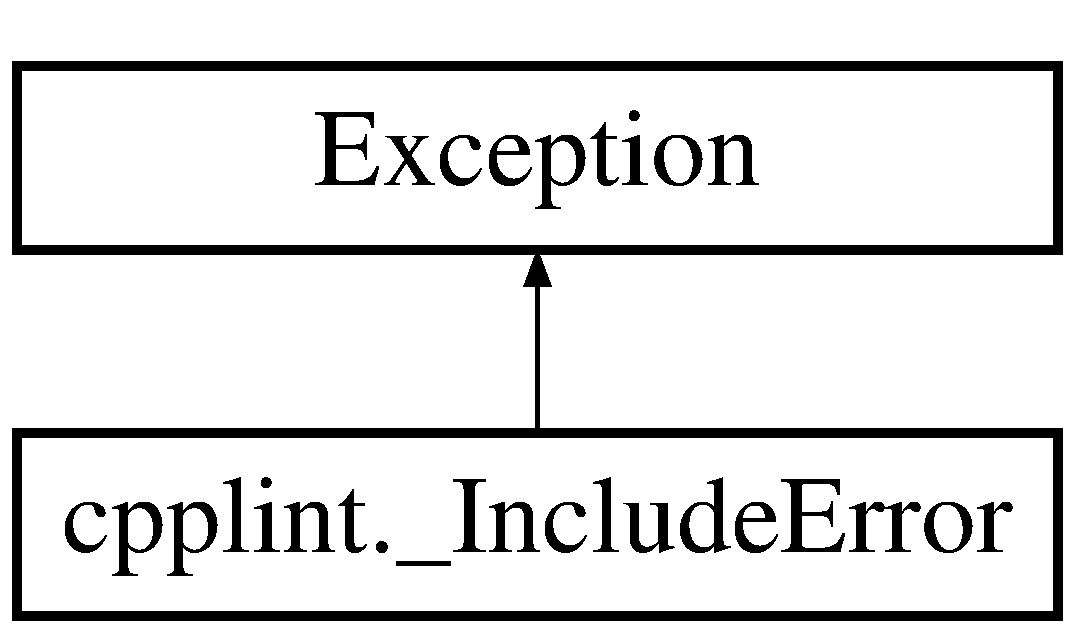
\includegraphics[height=2.000000cm]{classcpplint_1_1__IncludeError}
\end{center}
\end{figure}


\subsection{Detailed Description}
\begin{DoxyVerb}Indicates a problem with the include order in a file.\end{DoxyVerb}
 

The documentation for this class was generated from the following file\+:\begin{DoxyCompactItemize}
\item 
cpplint.\+py\end{DoxyCompactItemize}

\hypertarget{classcpplint_1_1__IncludeState}{}\section{cpplint.\+\_\+\+Include\+State Class Reference}
\label{classcpplint_1_1__IncludeState}\index{cpplint.\+\_\+\+Include\+State@{cpplint.\+\_\+\+Include\+State}}
Inheritance diagram for cpplint.\+\_\+\+Include\+State\+:\begin{figure}[H]
\begin{center}
\leavevmode
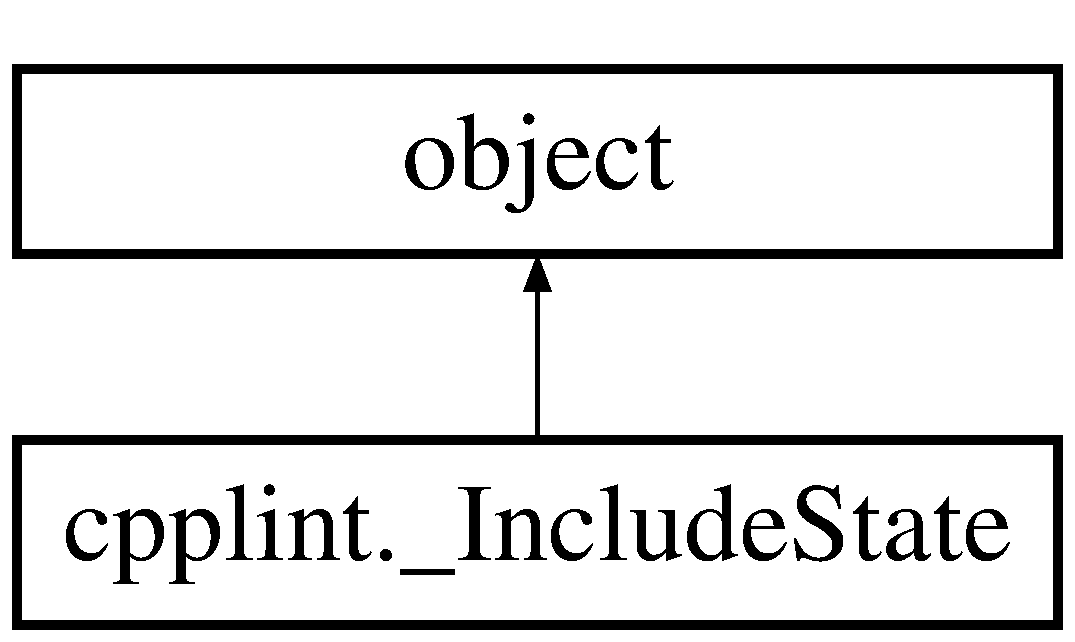
\includegraphics[height=2.000000cm]{classcpplint_1_1__IncludeState}
\end{center}
\end{figure}
\subsection*{Public Member Functions}
\begin{DoxyCompactItemize}
\item 
def {\bfseries \+\_\+\+\_\+init\+\_\+\+\_\+} (self)\hypertarget{classcpplint_1_1__IncludeState_a4d3ae4ee2a38efc25cce07e3e8484ba4}{}\label{classcpplint_1_1__IncludeState_a4d3ae4ee2a38efc25cce07e3e8484ba4}

\item 
def \hyperlink{classcpplint_1_1__IncludeState_a9bddbf581fc7a4c3c0258eaa42b94c3a}{Find\+Header} (self, header)
\item 
def \hyperlink{classcpplint_1_1__IncludeState_a31551f83fcc626e7babb1581a486b6fa}{Reset\+Section} (self, directive)
\item 
def {\bfseries Set\+Last\+Header} (self, header\+\_\+path)\hypertarget{classcpplint_1_1__IncludeState_a9bc1ada2060a49628c1fffa973b57df1}{}\label{classcpplint_1_1__IncludeState_a9bc1ada2060a49628c1fffa973b57df1}

\item 
def \hyperlink{classcpplint_1_1__IncludeState_ae69c652befa2d160194c0a02ff0c7d48}{Canonicalize\+Alphabetical\+Order} (self, header\+\_\+path)
\item 
def \hyperlink{classcpplint_1_1__IncludeState_abfda27324121ab0bf9d29866d975274b}{Is\+In\+Alphabetical\+Order} (self, clean\+\_\+lines, linenum, header\+\_\+path)
\item 
def \hyperlink{classcpplint_1_1__IncludeState_a80f82f17565e8412e7e5bbe52b464f18}{Check\+Next\+Include\+Order} (self, header\+\_\+type)
\end{DoxyCompactItemize}
\subsection*{Public Attributes}
\begin{DoxyCompactItemize}
\item 
{\bfseries include\+\_\+list}\hypertarget{classcpplint_1_1__IncludeState_a82d8b92a431437ee181e950517c71cbb}{}\label{classcpplint_1_1__IncludeState_a82d8b92a431437ee181e950517c71cbb}

\end{DoxyCompactItemize}


\subsection{Detailed Description}
\begin{DoxyVerb}Tracks line numbers for includes, and the order in which includes appear.

include_list contains list of lists of (header, line number) pairs.
It's a lists of lists rather than just one flat list to make it
easier to update across preprocessor boundaries.

Call CheckNextIncludeOrder() once for each header in the file, passing
in the type constants defined above. Calls in an illegal order will
raise an _IncludeError with an appropriate error message.\end{DoxyVerb}
 

\subsection{Member Function Documentation}
\index{cpplint\+::\+\_\+\+Include\+State@{cpplint\+::\+\_\+\+Include\+State}!Canonicalize\+Alphabetical\+Order@{Canonicalize\+Alphabetical\+Order}}
\index{Canonicalize\+Alphabetical\+Order@{Canonicalize\+Alphabetical\+Order}!cpplint\+::\+\_\+\+Include\+State@{cpplint\+::\+\_\+\+Include\+State}}
\subsubsection[{\texorpdfstring{Canonicalize\+Alphabetical\+Order(self, header\+\_\+path)}{CanonicalizeAlphabeticalOrder(self, header\_path)}}]{\setlength{\rightskip}{0pt plus 5cm}def cpplint.\+\_\+\+Include\+State.\+Canonicalize\+Alphabetical\+Order (
\begin{DoxyParamCaption}
\item[{}]{self, }
\item[{}]{header\+\_\+path}
\end{DoxyParamCaption}
)}\hypertarget{classcpplint_1_1__IncludeState_ae69c652befa2d160194c0a02ff0c7d48}{}\label{classcpplint_1_1__IncludeState_ae69c652befa2d160194c0a02ff0c7d48}
\begin{DoxyVerb}Returns a path canonicalized for alphabetical comparison.

- replaces "-" with "_" so they both cmp the same.
- removes '-inl' since we don't require them to be after the main header.
- lowercase everything, just in case.

Args:
  header_path: Path to be canonicalized.

Returns:
  Canonicalized path.
\end{DoxyVerb}
 \index{cpplint\+::\+\_\+\+Include\+State@{cpplint\+::\+\_\+\+Include\+State}!Check\+Next\+Include\+Order@{Check\+Next\+Include\+Order}}
\index{Check\+Next\+Include\+Order@{Check\+Next\+Include\+Order}!cpplint\+::\+\_\+\+Include\+State@{cpplint\+::\+\_\+\+Include\+State}}
\subsubsection[{\texorpdfstring{Check\+Next\+Include\+Order(self, header\+\_\+type)}{CheckNextIncludeOrder(self, header\_type)}}]{\setlength{\rightskip}{0pt plus 5cm}def cpplint.\+\_\+\+Include\+State.\+Check\+Next\+Include\+Order (
\begin{DoxyParamCaption}
\item[{}]{self, }
\item[{}]{header\+\_\+type}
\end{DoxyParamCaption}
)}\hypertarget{classcpplint_1_1__IncludeState_a80f82f17565e8412e7e5bbe52b464f18}{}\label{classcpplint_1_1__IncludeState_a80f82f17565e8412e7e5bbe52b464f18}
\begin{DoxyVerb}Returns a non-empty error message if the next header is out of order.

This function also updates the internal state to be ready to check
the next include.

Args:
  header_type: One of the _XXX_HEADER constants defined above.

Returns:
  The empty string if the header is in the right order, or an
  error message describing what's wrong.\end{DoxyVerb}
 \index{cpplint\+::\+\_\+\+Include\+State@{cpplint\+::\+\_\+\+Include\+State}!Find\+Header@{Find\+Header}}
\index{Find\+Header@{Find\+Header}!cpplint\+::\+\_\+\+Include\+State@{cpplint\+::\+\_\+\+Include\+State}}
\subsubsection[{\texorpdfstring{Find\+Header(self, header)}{FindHeader(self, header)}}]{\setlength{\rightskip}{0pt plus 5cm}def cpplint.\+\_\+\+Include\+State.\+Find\+Header (
\begin{DoxyParamCaption}
\item[{}]{self, }
\item[{}]{header}
\end{DoxyParamCaption}
)}\hypertarget{classcpplint_1_1__IncludeState_a9bddbf581fc7a4c3c0258eaa42b94c3a}{}\label{classcpplint_1_1__IncludeState_a9bddbf581fc7a4c3c0258eaa42b94c3a}
\begin{DoxyVerb}Check if a header has already been included.

Args:
  header: header to check.
Returns:
  Line number of previous occurrence, or -1 if the header has not
  been seen before.
\end{DoxyVerb}
 \index{cpplint\+::\+\_\+\+Include\+State@{cpplint\+::\+\_\+\+Include\+State}!Is\+In\+Alphabetical\+Order@{Is\+In\+Alphabetical\+Order}}
\index{Is\+In\+Alphabetical\+Order@{Is\+In\+Alphabetical\+Order}!cpplint\+::\+\_\+\+Include\+State@{cpplint\+::\+\_\+\+Include\+State}}
\subsubsection[{\texorpdfstring{Is\+In\+Alphabetical\+Order(self, clean\+\_\+lines, linenum, header\+\_\+path)}{IsInAlphabeticalOrder(self, clean\_lines, linenum, header\_path)}}]{\setlength{\rightskip}{0pt plus 5cm}def cpplint.\+\_\+\+Include\+State.\+Is\+In\+Alphabetical\+Order (
\begin{DoxyParamCaption}
\item[{}]{self, }
\item[{}]{clean\+\_\+lines, }
\item[{}]{linenum, }
\item[{}]{header\+\_\+path}
\end{DoxyParamCaption}
)}\hypertarget{classcpplint_1_1__IncludeState_abfda27324121ab0bf9d29866d975274b}{}\label{classcpplint_1_1__IncludeState_abfda27324121ab0bf9d29866d975274b}
\begin{DoxyVerb}Check if a header is in alphabetical order with the previous header.

Args:
  clean_lines: A CleansedLines instance containing the file.
  linenum: The number of the line to check.
  header_path: Canonicalized header to be checked.

Returns:
  Returns true if the header is in alphabetical order.
\end{DoxyVerb}
 \index{cpplint\+::\+\_\+\+Include\+State@{cpplint\+::\+\_\+\+Include\+State}!Reset\+Section@{Reset\+Section}}
\index{Reset\+Section@{Reset\+Section}!cpplint\+::\+\_\+\+Include\+State@{cpplint\+::\+\_\+\+Include\+State}}
\subsubsection[{\texorpdfstring{Reset\+Section(self, directive)}{ResetSection(self, directive)}}]{\setlength{\rightskip}{0pt plus 5cm}def cpplint.\+\_\+\+Include\+State.\+Reset\+Section (
\begin{DoxyParamCaption}
\item[{}]{self, }
\item[{}]{directive}
\end{DoxyParamCaption}
)}\hypertarget{classcpplint_1_1__IncludeState_a31551f83fcc626e7babb1581a486b6fa}{}\label{classcpplint_1_1__IncludeState_a31551f83fcc626e7babb1581a486b6fa}
\begin{DoxyVerb}Reset section checking for preprocessor directive.

Args:
  directive: preprocessor directive (e.g. "if", "else").
\end{DoxyVerb}
 

The documentation for this class was generated from the following file\+:\begin{DoxyCompactItemize}
\item 
cpplint.\+py\end{DoxyCompactItemize}

\hypertarget{classcpplint_1_1__NamespaceInfo}{}\section{cpplint.\+\_\+\+Namespace\+Info Class Reference}
\label{classcpplint_1_1__NamespaceInfo}\index{cpplint.\+\_\+\+Namespace\+Info@{cpplint.\+\_\+\+Namespace\+Info}}
Inheritance diagram for cpplint.\+\_\+\+Namespace\+Info\+:\begin{figure}[H]
\begin{center}
\leavevmode
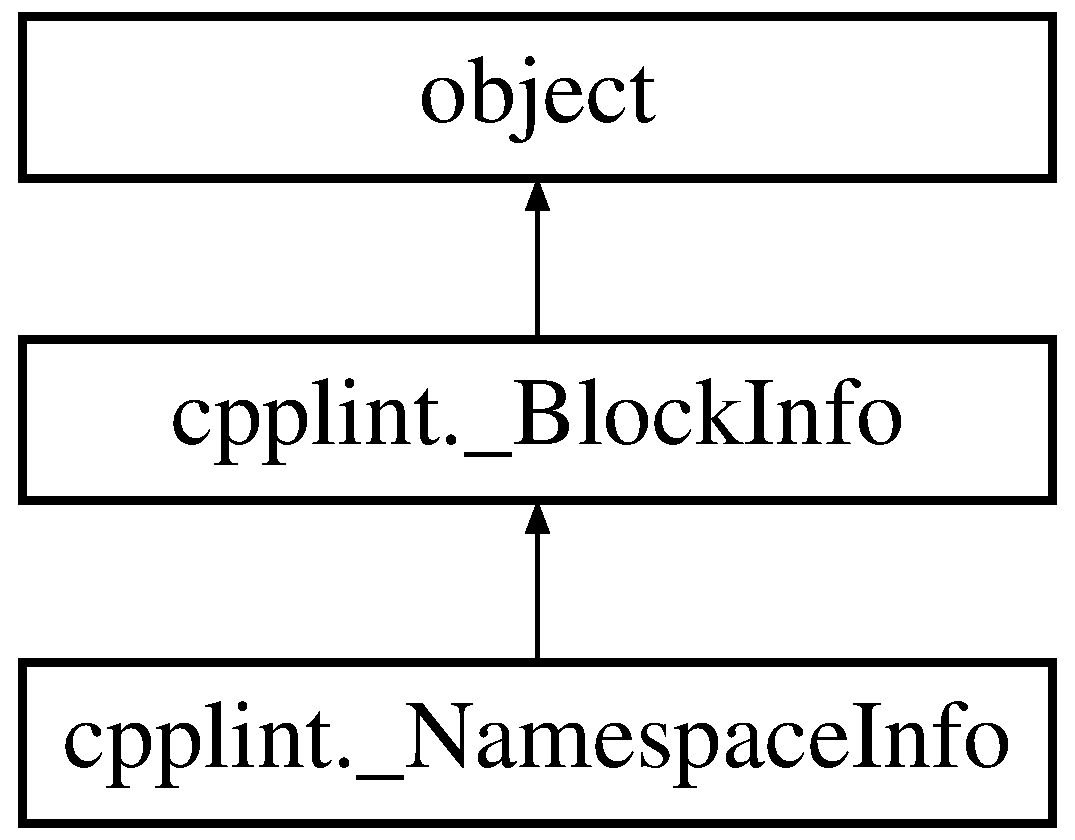
\includegraphics[height=3.000000cm]{classcpplint_1_1__NamespaceInfo}
\end{center}
\end{figure}
\subsection*{Public Member Functions}
\begin{DoxyCompactItemize}
\item 
def {\bfseries \+\_\+\+\_\+init\+\_\+\+\_\+} (self, name, linenum)\hypertarget{classcpplint_1_1__NamespaceInfo_a4425c93bd90fbf869dc31c87302f5bb0}{}\label{classcpplint_1_1__NamespaceInfo_a4425c93bd90fbf869dc31c87302f5bb0}

\item 
def \hyperlink{classcpplint_1_1__NamespaceInfo_a9d3abaeed0353942ca689eeeb2f2924b}{Check\+End} (self, filename, clean\+\_\+lines, linenum, error)
\end{DoxyCompactItemize}
\subsection*{Public Attributes}
\begin{DoxyCompactItemize}
\item 
{\bfseries name}\hypertarget{classcpplint_1_1__NamespaceInfo_a6b518dae822e4e440405654e83dc86a1}{}\label{classcpplint_1_1__NamespaceInfo_a6b518dae822e4e440405654e83dc86a1}

\item 
{\bfseries starting\+\_\+linenum}\hypertarget{classcpplint_1_1__NamespaceInfo_a1053c0f6e43847a24774ace88b9f5719}{}\label{classcpplint_1_1__NamespaceInfo_a1053c0f6e43847a24774ace88b9f5719}

\item 
{\bfseries check\+\_\+namespace\+\_\+indentation}\hypertarget{classcpplint_1_1__NamespaceInfo_ae0b0b6ffafd3336a93cddca1078df268}{}\label{classcpplint_1_1__NamespaceInfo_ae0b0b6ffafd3336a93cddca1078df268}

\end{DoxyCompactItemize}


\subsection{Detailed Description}
\begin{DoxyVerb}Stores information about a namespace.\end{DoxyVerb}
 

\subsection{Member Function Documentation}
\index{cpplint\+::\+\_\+\+Namespace\+Info@{cpplint\+::\+\_\+\+Namespace\+Info}!Check\+End@{Check\+End}}
\index{Check\+End@{Check\+End}!cpplint\+::\+\_\+\+Namespace\+Info@{cpplint\+::\+\_\+\+Namespace\+Info}}
\subsubsection[{\texorpdfstring{Check\+End(self, filename, clean\+\_\+lines, linenum, error)}{CheckEnd(self, filename, clean\_lines, linenum, error)}}]{\setlength{\rightskip}{0pt plus 5cm}def cpplint.\+\_\+\+Namespace\+Info.\+Check\+End (
\begin{DoxyParamCaption}
\item[{}]{self, }
\item[{}]{filename, }
\item[{}]{clean\+\_\+lines, }
\item[{}]{linenum, }
\item[{}]{error}
\end{DoxyParamCaption}
)}\hypertarget{classcpplint_1_1__NamespaceInfo_a9d3abaeed0353942ca689eeeb2f2924b}{}\label{classcpplint_1_1__NamespaceInfo_a9d3abaeed0353942ca689eeeb2f2924b}
\begin{DoxyVerb}Check end of namespace comments.\end{DoxyVerb}
 

The documentation for this class was generated from the following file\+:\begin{DoxyCompactItemize}
\item 
cpplint.\+py\end{DoxyCompactItemize}

\hypertarget{classcpplint_1_1__PreprocessorInfo}{}\section{cpplint.\+\_\+\+Preprocessor\+Info Class Reference}
\label{classcpplint_1_1__PreprocessorInfo}\index{cpplint.\+\_\+\+Preprocessor\+Info@{cpplint.\+\_\+\+Preprocessor\+Info}}
Inheritance diagram for cpplint.\+\_\+\+Preprocessor\+Info\+:\begin{figure}[H]
\begin{center}
\leavevmode
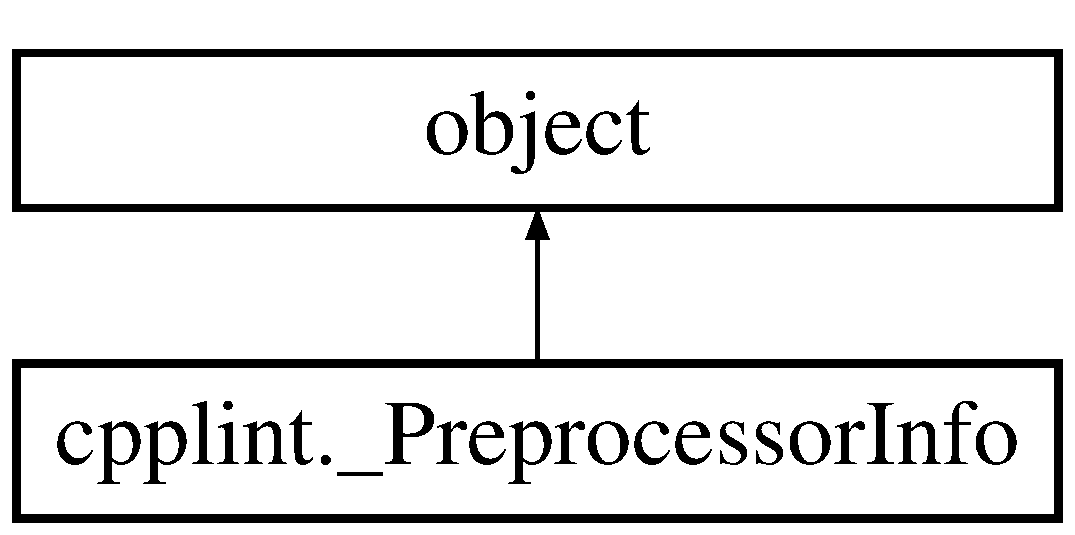
\includegraphics[height=2.000000cm]{classcpplint_1_1__PreprocessorInfo}
\end{center}
\end{figure}
\subsection*{Public Member Functions}
\begin{DoxyCompactItemize}
\item 
def {\bfseries \+\_\+\+\_\+init\+\_\+\+\_\+} (self, stack\+\_\+before\+\_\+if)\hypertarget{classcpplint_1_1__PreprocessorInfo_a1394d17434a22d32b0ea9d6424e5c47b}{}\label{classcpplint_1_1__PreprocessorInfo_a1394d17434a22d32b0ea9d6424e5c47b}

\end{DoxyCompactItemize}
\subsection*{Public Attributes}
\begin{DoxyCompactItemize}
\item 
{\bfseries stack\+\_\+before\+\_\+if}\hypertarget{classcpplint_1_1__PreprocessorInfo_a0681b2adca3171a495fc1eca43d245c0}{}\label{classcpplint_1_1__PreprocessorInfo_a0681b2adca3171a495fc1eca43d245c0}

\item 
{\bfseries stack\+\_\+before\+\_\+else}\hypertarget{classcpplint_1_1__PreprocessorInfo_a34a80f1f97808614b7062ba1e5bbf2b9}{}\label{classcpplint_1_1__PreprocessorInfo_a34a80f1f97808614b7062ba1e5bbf2b9}

\item 
{\bfseries seen\+\_\+else}\hypertarget{classcpplint_1_1__PreprocessorInfo_a7587e84a1e6db34c3c94317f5a5931cc}{}\label{classcpplint_1_1__PreprocessorInfo_a7587e84a1e6db34c3c94317f5a5931cc}

\end{DoxyCompactItemize}


\subsection{Detailed Description}
\begin{DoxyVerb}Stores checkpoints of nesting stacks when #if/#else is seen.\end{DoxyVerb}
 

The documentation for this class was generated from the following file\+:\begin{DoxyCompactItemize}
\item 
cpplint.\+py\end{DoxyCompactItemize}

\hypertarget{classBattery}{}\section{Battery Class Reference}
\label{classBattery}\index{Battery@{Battery}}


{\ttfamily \#include $<$battery.\+h$>$}

\subsection*{Public Member Functions}
\begin{DoxyCompactItemize}
\item 
double \hyperlink{classBattery_a8a21d21a6bcac4eede5ce0ff5e0f2a2b}{get\+Charge} (void)
\item 
void \hyperlink{classBattery_af20b927a6d29efa1aac61f00757fafdd}{add\+To\+Charge} (double power)
\item 
void \hyperlink{classBattery_a4cfef00a4bd5a31a66b5a20d06179e1c}{subtract\+From\+Charge} (double power)
\item 
\hyperlink{classBattery_a36a6234c583e3b3506f4a77e3eb49989}{Battery} ()
\item 
\hyperlink{classBattery_a40c4232556ff1516ff06056d422fa641}{Battery} (double initial\+Charge)
\end{DoxyCompactItemize}


\subsection{Detailed Description}
Stores the amount of charge in a battery and provides methods to add charge, subtract charge, and get charge 

\subsection{Constructor \& Destructor Documentation}
\index{Battery@{Battery}!Battery@{Battery}}
\index{Battery@{Battery}!Battery@{Battery}}
\subsubsection[{\texorpdfstring{Battery()}{Battery()}}]{\setlength{\rightskip}{0pt plus 5cm}Battery\+::\+Battery (
\begin{DoxyParamCaption}
\item[{void}]{}
\end{DoxyParamCaption}
)}\hypertarget{classBattery_a36a6234c583e3b3506f4a77e3eb49989}{}\label{classBattery_a36a6234c583e3b3506f4a77e3eb49989}
Creates a battery object \index{Battery@{Battery}!Battery@{Battery}}
\index{Battery@{Battery}!Battery@{Battery}}
\subsubsection[{\texorpdfstring{Battery(double initial\+Charge)}{Battery(double initialCharge)}}]{\setlength{\rightskip}{0pt plus 5cm}Battery\+::\+Battery (
\begin{DoxyParamCaption}
\item[{double}]{initial\+Charge}
\end{DoxyParamCaption}
)\hspace{0.3cm}{\ttfamily [explicit]}}\hypertarget{classBattery_a40c4232556ff1516ff06056d422fa641}{}\label{classBattery_a40c4232556ff1516ff06056d422fa641}
Creates a bettery object with a charge


\begin{DoxyParams}{Parameters}
{\em initial\+Charge} & The initial charge of the battery \\
\hline
\end{DoxyParams}


\subsection{Member Function Documentation}
\index{Battery@{Battery}!add\+To\+Charge@{add\+To\+Charge}}
\index{add\+To\+Charge@{add\+To\+Charge}!Battery@{Battery}}
\subsubsection[{\texorpdfstring{add\+To\+Charge(double power)}{addToCharge(double power)}}]{\setlength{\rightskip}{0pt plus 5cm}void Battery\+::add\+To\+Charge (
\begin{DoxyParamCaption}
\item[{double}]{power}
\end{DoxyParamCaption}
)}\hypertarget{classBattery_af20b927a6d29efa1aac61f00757fafdd}{}\label{classBattery_af20b927a6d29efa1aac61f00757fafdd}
Adds a specified amount of charge to the battery


\begin{DoxyParams}{Parameters}
{\em power} & The amount of charge to add. \\
\hline
\end{DoxyParams}
\index{Battery@{Battery}!get\+Charge@{get\+Charge}}
\index{get\+Charge@{get\+Charge}!Battery@{Battery}}
\subsubsection[{\texorpdfstring{get\+Charge(void)}{getCharge(void)}}]{\setlength{\rightskip}{0pt plus 5cm}double Battery\+::get\+Charge (
\begin{DoxyParamCaption}
\item[{void}]{}
\end{DoxyParamCaption}
)}\hypertarget{classBattery_a8a21d21a6bcac4eede5ce0ff5e0f2a2b}{}\label{classBattery_a8a21d21a6bcac4eede5ce0ff5e0f2a2b}
Returns how much charge is in the battery

\begin{DoxyReturn}{Returns}
The amount of charge in the battery. 
\end{DoxyReturn}
\index{Battery@{Battery}!subtract\+From\+Charge@{subtract\+From\+Charge}}
\index{subtract\+From\+Charge@{subtract\+From\+Charge}!Battery@{Battery}}
\subsubsection[{\texorpdfstring{subtract\+From\+Charge(double power)}{subtractFromCharge(double power)}}]{\setlength{\rightskip}{0pt plus 5cm}void Battery\+::subtract\+From\+Charge (
\begin{DoxyParamCaption}
\item[{double}]{power}
\end{DoxyParamCaption}
)}\hypertarget{classBattery_a4cfef00a4bd5a31a66b5a20d06179e1c}{}\label{classBattery_a4cfef00a4bd5a31a66b5a20d06179e1c}
Subtracts a specified amount of charge from the battery


\begin{DoxyParams}{Parameters}
{\em power} & The amount of charge to subtract \\
\hline
\end{DoxyParams}


The documentation for this class was generated from the following files\+:\begin{DoxyCompactItemize}
\item 
\hyperlink{battery_8h}{battery.\+h}\item 
\hyperlink{battery_8cpp}{battery.\+cpp}\end{DoxyCompactItemize}

\hypertarget{classcpplint_1_1CleansedLines}{}\section{cpplint.\+Cleansed\+Lines Class Reference}
\label{classcpplint_1_1CleansedLines}\index{cpplint.\+Cleansed\+Lines@{cpplint.\+Cleansed\+Lines}}
Inheritance diagram for cpplint.\+Cleansed\+Lines\+:\begin{figure}[H]
\begin{center}
\leavevmode
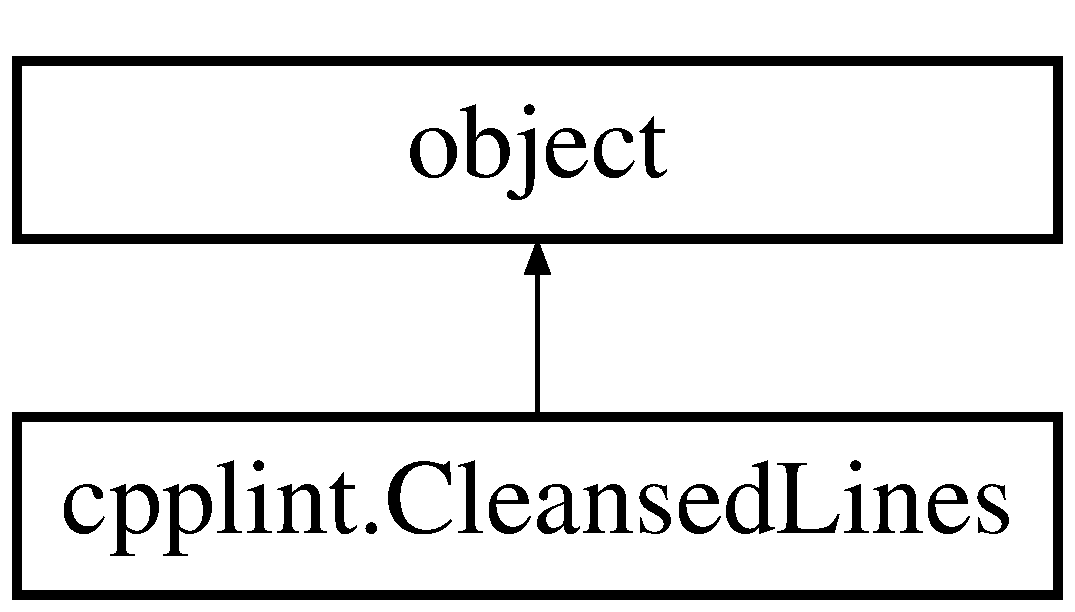
\includegraphics[height=2.000000cm]{classcpplint_1_1CleansedLines}
\end{center}
\end{figure}
\subsection*{Public Member Functions}
\begin{DoxyCompactItemize}
\item 
def {\bfseries \+\_\+\+\_\+init\+\_\+\+\_\+} (self, lines)\hypertarget{classcpplint_1_1CleansedLines_ad2bc06d9697e2bbfbc7e6b50878c8c8f}{}\label{classcpplint_1_1CleansedLines_ad2bc06d9697e2bbfbc7e6b50878c8c8f}

\item 
def \hyperlink{classcpplint_1_1CleansedLines_a26a7eff70493d64d58d16f4a406c7ee9}{Num\+Lines} (self)
\end{DoxyCompactItemize}
\subsection*{Public Attributes}
\begin{DoxyCompactItemize}
\item 
{\bfseries elided}\hypertarget{classcpplint_1_1CleansedLines_aa4d0a4d5081675c01656a5d86d99e8bd}{}\label{classcpplint_1_1CleansedLines_aa4d0a4d5081675c01656a5d86d99e8bd}

\item 
{\bfseries lines}\hypertarget{classcpplint_1_1CleansedLines_a9cd74bd010da1610a46322d6821bd06a}{}\label{classcpplint_1_1CleansedLines_a9cd74bd010da1610a46322d6821bd06a}

\item 
{\bfseries raw\+\_\+lines}\hypertarget{classcpplint_1_1CleansedLines_a9e94ce9e4f682be33c04fe82429c4dfd}{}\label{classcpplint_1_1CleansedLines_a9e94ce9e4f682be33c04fe82429c4dfd}

\item 
{\bfseries num\+\_\+lines}\hypertarget{classcpplint_1_1CleansedLines_a4b42ab48659954fb6e0a4e4eb483a45a}{}\label{classcpplint_1_1CleansedLines_a4b42ab48659954fb6e0a4e4eb483a45a}

\item 
{\bfseries lines\+\_\+without\+\_\+raw\+\_\+strings}\hypertarget{classcpplint_1_1CleansedLines_a0cc228ba3c00ba590b27a759cf8023ce}{}\label{classcpplint_1_1CleansedLines_a0cc228ba3c00ba590b27a759cf8023ce}

\end{DoxyCompactItemize}


\subsection{Detailed Description}
\begin{DoxyVerb}Holds 4 copies of all lines with different preprocessing applied to them.

1) elided member contains lines without strings and comments.
2) lines member contains lines without comments.
3) raw_lines member contains all the lines without processing.
4) lines_without_raw_strings member is same as raw_lines, but with C++11 raw
   strings removed.
All these members are of <type 'list'>, and of the same length.
\end{DoxyVerb}
 

\subsection{Member Function Documentation}
\index{cpplint\+::\+Cleansed\+Lines@{cpplint\+::\+Cleansed\+Lines}!Num\+Lines@{Num\+Lines}}
\index{Num\+Lines@{Num\+Lines}!cpplint\+::\+Cleansed\+Lines@{cpplint\+::\+Cleansed\+Lines}}
\subsubsection[{\texorpdfstring{Num\+Lines(self)}{NumLines(self)}}]{\setlength{\rightskip}{0pt plus 5cm}def cpplint.\+Cleansed\+Lines.\+Num\+Lines (
\begin{DoxyParamCaption}
\item[{}]{self}
\end{DoxyParamCaption}
)}\hypertarget{classcpplint_1_1CleansedLines_a26a7eff70493d64d58d16f4a406c7ee9}{}\label{classcpplint_1_1CleansedLines_a26a7eff70493d64d58d16f4a406c7ee9}
\begin{DoxyVerb}Returns the number of lines represented.\end{DoxyVerb}
 

The documentation for this class was generated from the following file\+:\begin{DoxyCompactItemize}
\item 
cpplint.\+py\end{DoxyCompactItemize}

\hypertarget{classcpplint_1_1FileInfo}{}\section{cpplint.\+File\+Info Class Reference}
\label{classcpplint_1_1FileInfo}\index{cpplint.\+File\+Info@{cpplint.\+File\+Info}}
Inheritance diagram for cpplint.\+File\+Info\+:\begin{figure}[H]
\begin{center}
\leavevmode
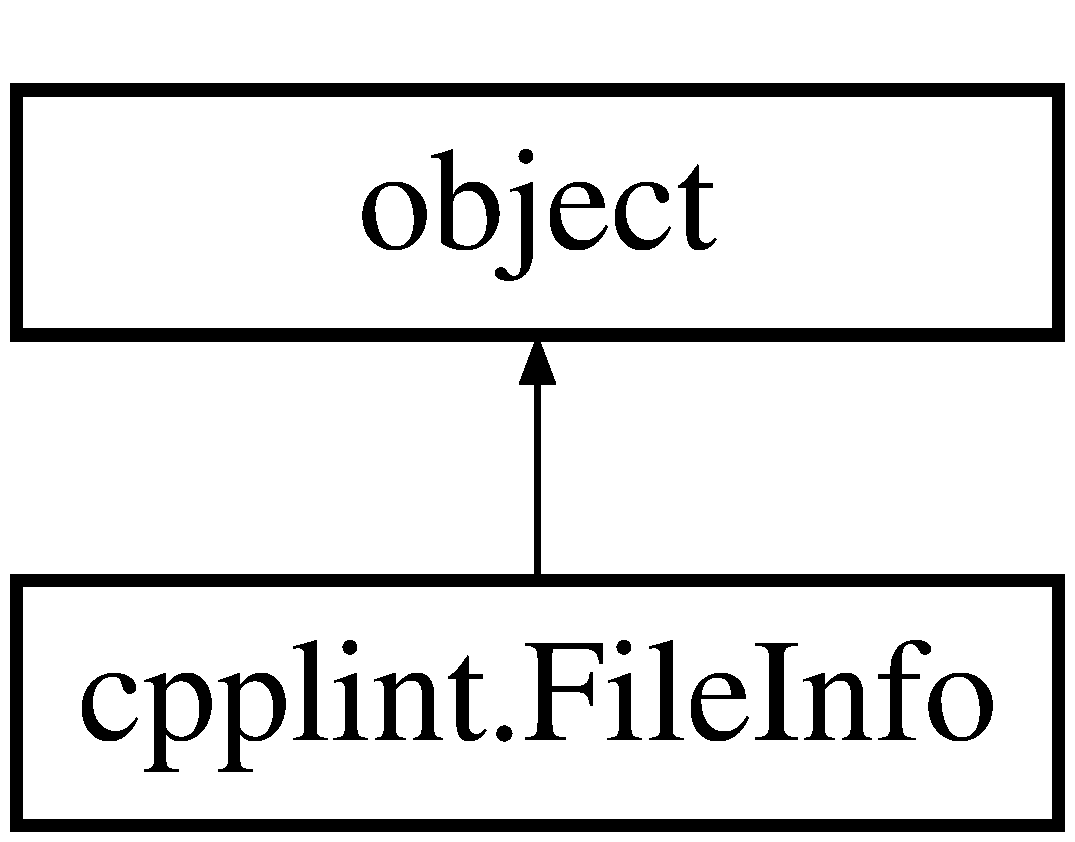
\includegraphics[height=2.000000cm]{classcpplint_1_1FileInfo}
\end{center}
\end{figure}
\subsection*{Public Member Functions}
\begin{DoxyCompactItemize}
\item 
def {\bfseries \+\_\+\+\_\+init\+\_\+\+\_\+} (self, filename)\hypertarget{classcpplint_1_1FileInfo_abd3ff77aab027af2476b3a1d97b1f89c}{}\label{classcpplint_1_1FileInfo_abd3ff77aab027af2476b3a1d97b1f89c}

\item 
def \hyperlink{classcpplint_1_1FileInfo_aed56577368c45cdf45fc4c9109129145}{Full\+Name} (self)
\item 
def \hyperlink{classcpplint_1_1FileInfo_a2b3b79b7d46221a6b9d0ea0bebac2061}{Repository\+Name} (self)
\item 
def \hyperlink{classcpplint_1_1FileInfo_a43f1c5ff1771da52e29c60c114955e72}{Split} (self)
\item 
def \hyperlink{classcpplint_1_1FileInfo_a1a12ed63ddc2ffd8f6a105e3ab4d6289}{Base\+Name} (self)
\item 
def \hyperlink{classcpplint_1_1FileInfo_a2554b504117839931e901b59a59c67ae}{Extension} (self)
\item 
def \hyperlink{classcpplint_1_1FileInfo_acb46555a72b346966f4bf28c08e3b1fa}{No\+Extension} (self)
\item 
def \hyperlink{classcpplint_1_1FileInfo_a157f8d3266d7291321db88cdad3b2879}{Is\+Source} (self)
\end{DoxyCompactItemize}


\subsection{Detailed Description}
\begin{DoxyVerb}Provides utility functions for filenames.

FileInfo provides easy access to the components of a file's path
relative to the project root.
\end{DoxyVerb}
 

\subsection{Member Function Documentation}
\index{cpplint\+::\+File\+Info@{cpplint\+::\+File\+Info}!Base\+Name@{Base\+Name}}
\index{Base\+Name@{Base\+Name}!cpplint\+::\+File\+Info@{cpplint\+::\+File\+Info}}
\subsubsection[{\texorpdfstring{Base\+Name(self)}{BaseName(self)}}]{\setlength{\rightskip}{0pt plus 5cm}def cpplint.\+File\+Info.\+Base\+Name (
\begin{DoxyParamCaption}
\item[{}]{self}
\end{DoxyParamCaption}
)}\hypertarget{classcpplint_1_1FileInfo_a1a12ed63ddc2ffd8f6a105e3ab4d6289}{}\label{classcpplint_1_1FileInfo_a1a12ed63ddc2ffd8f6a105e3ab4d6289}
\begin{DoxyVerb}File base name - text after the final slash, before the final period.\end{DoxyVerb}
 \index{cpplint\+::\+File\+Info@{cpplint\+::\+File\+Info}!Extension@{Extension}}
\index{Extension@{Extension}!cpplint\+::\+File\+Info@{cpplint\+::\+File\+Info}}
\subsubsection[{\texorpdfstring{Extension(self)}{Extension(self)}}]{\setlength{\rightskip}{0pt plus 5cm}def cpplint.\+File\+Info.\+Extension (
\begin{DoxyParamCaption}
\item[{}]{self}
\end{DoxyParamCaption}
)}\hypertarget{classcpplint_1_1FileInfo_a2554b504117839931e901b59a59c67ae}{}\label{classcpplint_1_1FileInfo_a2554b504117839931e901b59a59c67ae}
\begin{DoxyVerb}File extension - text following the final period.\end{DoxyVerb}
 \index{cpplint\+::\+File\+Info@{cpplint\+::\+File\+Info}!Full\+Name@{Full\+Name}}
\index{Full\+Name@{Full\+Name}!cpplint\+::\+File\+Info@{cpplint\+::\+File\+Info}}
\subsubsection[{\texorpdfstring{Full\+Name(self)}{FullName(self)}}]{\setlength{\rightskip}{0pt plus 5cm}def cpplint.\+File\+Info.\+Full\+Name (
\begin{DoxyParamCaption}
\item[{}]{self}
\end{DoxyParamCaption}
)}\hypertarget{classcpplint_1_1FileInfo_aed56577368c45cdf45fc4c9109129145}{}\label{classcpplint_1_1FileInfo_aed56577368c45cdf45fc4c9109129145}
\begin{DoxyVerb}Make Windows paths like Unix.\end{DoxyVerb}
 \index{cpplint\+::\+File\+Info@{cpplint\+::\+File\+Info}!Is\+Source@{Is\+Source}}
\index{Is\+Source@{Is\+Source}!cpplint\+::\+File\+Info@{cpplint\+::\+File\+Info}}
\subsubsection[{\texorpdfstring{Is\+Source(self)}{IsSource(self)}}]{\setlength{\rightskip}{0pt plus 5cm}def cpplint.\+File\+Info.\+Is\+Source (
\begin{DoxyParamCaption}
\item[{}]{self}
\end{DoxyParamCaption}
)}\hypertarget{classcpplint_1_1FileInfo_a157f8d3266d7291321db88cdad3b2879}{}\label{classcpplint_1_1FileInfo_a157f8d3266d7291321db88cdad3b2879}
\begin{DoxyVerb}File has a source file extension.\end{DoxyVerb}
 \index{cpplint\+::\+File\+Info@{cpplint\+::\+File\+Info}!No\+Extension@{No\+Extension}}
\index{No\+Extension@{No\+Extension}!cpplint\+::\+File\+Info@{cpplint\+::\+File\+Info}}
\subsubsection[{\texorpdfstring{No\+Extension(self)}{NoExtension(self)}}]{\setlength{\rightskip}{0pt plus 5cm}def cpplint.\+File\+Info.\+No\+Extension (
\begin{DoxyParamCaption}
\item[{}]{self}
\end{DoxyParamCaption}
)}\hypertarget{classcpplint_1_1FileInfo_acb46555a72b346966f4bf28c08e3b1fa}{}\label{classcpplint_1_1FileInfo_acb46555a72b346966f4bf28c08e3b1fa}
\begin{DoxyVerb}File has no source file extension.\end{DoxyVerb}
 \index{cpplint\+::\+File\+Info@{cpplint\+::\+File\+Info}!Repository\+Name@{Repository\+Name}}
\index{Repository\+Name@{Repository\+Name}!cpplint\+::\+File\+Info@{cpplint\+::\+File\+Info}}
\subsubsection[{\texorpdfstring{Repository\+Name(self)}{RepositoryName(self)}}]{\setlength{\rightskip}{0pt plus 5cm}def cpplint.\+File\+Info.\+Repository\+Name (
\begin{DoxyParamCaption}
\item[{}]{self}
\end{DoxyParamCaption}
)}\hypertarget{classcpplint_1_1FileInfo_a2b3b79b7d46221a6b9d0ea0bebac2061}{}\label{classcpplint_1_1FileInfo_a2b3b79b7d46221a6b9d0ea0bebac2061}
\begin{DoxyVerb}FullName after removing the local path to the repository.

If we have a real absolute path name here we can try to do something smart:
detecting the root of the checkout and truncating /path/to/checkout from
the name so that we get header guards that don't include things like
"C:\Documents and Settings\..." or "/home/username/..." in them and thus
people on different computers who have checked the source out to different
locations won't see bogus errors.
\end{DoxyVerb}
 \index{cpplint\+::\+File\+Info@{cpplint\+::\+File\+Info}!Split@{Split}}
\index{Split@{Split}!cpplint\+::\+File\+Info@{cpplint\+::\+File\+Info}}
\subsubsection[{\texorpdfstring{Split(self)}{Split(self)}}]{\setlength{\rightskip}{0pt plus 5cm}def cpplint.\+File\+Info.\+Split (
\begin{DoxyParamCaption}
\item[{}]{self}
\end{DoxyParamCaption}
)}\hypertarget{classcpplint_1_1FileInfo_a43f1c5ff1771da52e29c60c114955e72}{}\label{classcpplint_1_1FileInfo_a43f1c5ff1771da52e29c60c114955e72}
\begin{DoxyVerb}Splits the file into the directory, basename, and extension.

For 'chrome/browser/browser.cc', Split() would
return ('chrome/browser', 'browser', '.cc')

Returns:
  A tuple of (directory, basename, extension).
\end{DoxyVerb}
 

The documentation for this class was generated from the following file\+:\begin{DoxyCompactItemize}
\item 
cpplint.\+py\end{DoxyCompactItemize}

\hypertarget{classcpplint_1_1NestingState}{}\section{cpplint.\+Nesting\+State Class Reference}
\label{classcpplint_1_1NestingState}\index{cpplint.\+Nesting\+State@{cpplint.\+Nesting\+State}}
Inheritance diagram for cpplint.\+Nesting\+State\+:\begin{figure}[H]
\begin{center}
\leavevmode
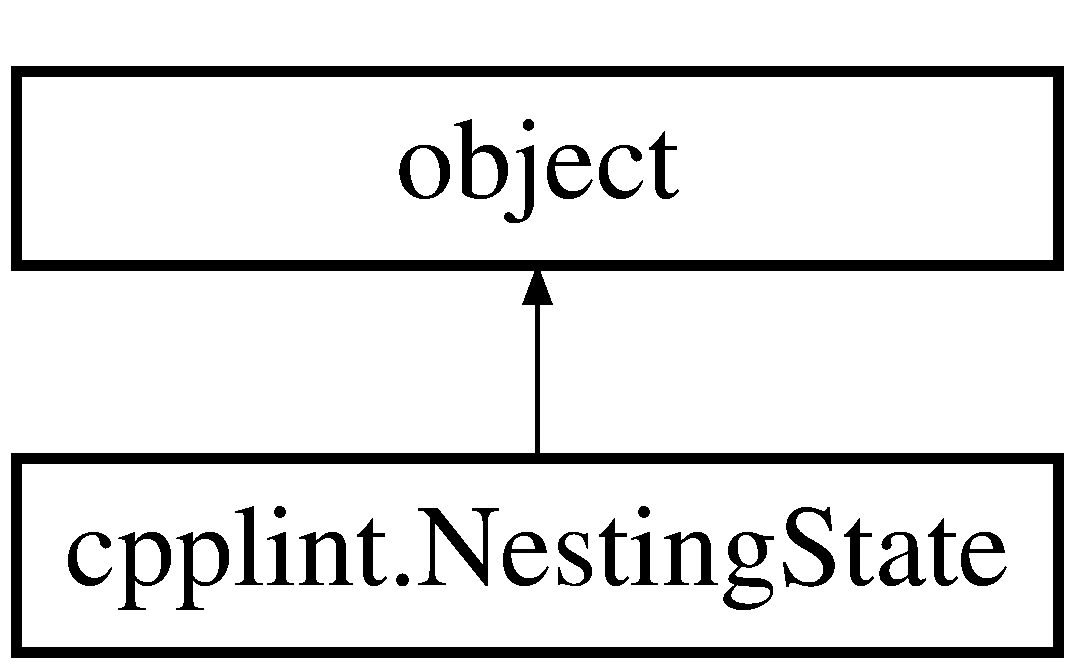
\includegraphics[height=2.000000cm]{classcpplint_1_1NestingState}
\end{center}
\end{figure}
\subsection*{Public Member Functions}
\begin{DoxyCompactItemize}
\item 
def {\bfseries \+\_\+\+\_\+init\+\_\+\+\_\+} (self)\hypertarget{classcpplint_1_1NestingState_a47e1ad559b9c7304f53d19ef6ebedab4}{}\label{classcpplint_1_1NestingState_a47e1ad559b9c7304f53d19ef6ebedab4}

\item 
def \hyperlink{classcpplint_1_1NestingState_a15abc0719a22ca8fbb7a8235f0e22b3e}{Seen\+Open\+Brace} (self)
\item 
def \hyperlink{classcpplint_1_1NestingState_a1a06f50d53cfe11b1f78d45b531e0c32}{In\+Namespace\+Body} (self)
\item 
def \hyperlink{classcpplint_1_1NestingState_a67aa1907d42b8408c227ff18537071c7}{In\+ExternC} (self)
\item 
def \hyperlink{classcpplint_1_1NestingState_a8e111c25149c41bd8927606244965b3c}{In\+Class\+Declaration} (self)
\item 
def \hyperlink{classcpplint_1_1NestingState_aa35a529052e4863a477eae649ce778d2}{In\+Asm\+Block} (self)
\item 
def \hyperlink{classcpplint_1_1NestingState_a8f4e9ba1aaa0459de2bedd966e7a2b54}{In\+Template\+Argument\+List} (self, clean\+\_\+lines, linenum, pos)
\item 
def \hyperlink{classcpplint_1_1NestingState_ac3d509c536af445e8ab6b17b067b53f1}{Update\+Preprocessor} (self, line)
\item 
def \hyperlink{classcpplint_1_1NestingState_a3adead8c1575b98ace5c5230f3772c1e}{Update} (self, filename, clean\+\_\+lines, linenum, error)
\item 
def \hyperlink{classcpplint_1_1NestingState_a4141768e75b16698463670caaa587120}{Innermost\+Class} (self)
\item 
def \hyperlink{classcpplint_1_1NestingState_a7bde5ab65152b4073763b1bd17cba567}{Check\+Completed\+Blocks} (self, filename, error)
\end{DoxyCompactItemize}
\subsection*{Public Attributes}
\begin{DoxyCompactItemize}
\item 
{\bfseries stack}\hypertarget{classcpplint_1_1NestingState_a6ae9bea040f988d152922788d0d73a15}{}\label{classcpplint_1_1NestingState_a6ae9bea040f988d152922788d0d73a15}

\item 
{\bfseries previous\+\_\+stack\+\_\+top}\hypertarget{classcpplint_1_1NestingState_a7aa34c8fb8df73d76f702c7012c46911}{}\label{classcpplint_1_1NestingState_a7aa34c8fb8df73d76f702c7012c46911}

\item 
{\bfseries pp\+\_\+stack}\hypertarget{classcpplint_1_1NestingState_a3a5ca37e3066d91830ea1faa8feae4e5}{}\label{classcpplint_1_1NestingState_a3a5ca37e3066d91830ea1faa8feae4e5}

\end{DoxyCompactItemize}


\subsection{Detailed Description}
\begin{DoxyVerb}Holds states related to parsing braces.\end{DoxyVerb}
 

\subsection{Member Function Documentation}
\index{cpplint\+::\+Nesting\+State@{cpplint\+::\+Nesting\+State}!Check\+Completed\+Blocks@{Check\+Completed\+Blocks}}
\index{Check\+Completed\+Blocks@{Check\+Completed\+Blocks}!cpplint\+::\+Nesting\+State@{cpplint\+::\+Nesting\+State}}
\subsubsection[{\texorpdfstring{Check\+Completed\+Blocks(self, filename, error)}{CheckCompletedBlocks(self, filename, error)}}]{\setlength{\rightskip}{0pt plus 5cm}def cpplint.\+Nesting\+State.\+Check\+Completed\+Blocks (
\begin{DoxyParamCaption}
\item[{}]{self, }
\item[{}]{filename, }
\item[{}]{error}
\end{DoxyParamCaption}
)}\hypertarget{classcpplint_1_1NestingState_a7bde5ab65152b4073763b1bd17cba567}{}\label{classcpplint_1_1NestingState_a7bde5ab65152b4073763b1bd17cba567}
\begin{DoxyVerb}Checks that all classes and namespaces have been completely parsed.

Call this when all lines in a file have been processed.
Args:
  filename: The name of the current file.
  error: The function to call with any errors found.
\end{DoxyVerb}
 \index{cpplint\+::\+Nesting\+State@{cpplint\+::\+Nesting\+State}!In\+Asm\+Block@{In\+Asm\+Block}}
\index{In\+Asm\+Block@{In\+Asm\+Block}!cpplint\+::\+Nesting\+State@{cpplint\+::\+Nesting\+State}}
\subsubsection[{\texorpdfstring{In\+Asm\+Block(self)}{InAsmBlock(self)}}]{\setlength{\rightskip}{0pt plus 5cm}def cpplint.\+Nesting\+State.\+In\+Asm\+Block (
\begin{DoxyParamCaption}
\item[{}]{self}
\end{DoxyParamCaption}
)}\hypertarget{classcpplint_1_1NestingState_aa35a529052e4863a477eae649ce778d2}{}\label{classcpplint_1_1NestingState_aa35a529052e4863a477eae649ce778d2}
\begin{DoxyVerb}Check if we are currently one level inside an inline ASM block.

Returns:
  True if the top of the stack is a block containing inline ASM.
\end{DoxyVerb}
 \index{cpplint\+::\+Nesting\+State@{cpplint\+::\+Nesting\+State}!In\+Class\+Declaration@{In\+Class\+Declaration}}
\index{In\+Class\+Declaration@{In\+Class\+Declaration}!cpplint\+::\+Nesting\+State@{cpplint\+::\+Nesting\+State}}
\subsubsection[{\texorpdfstring{In\+Class\+Declaration(self)}{InClassDeclaration(self)}}]{\setlength{\rightskip}{0pt plus 5cm}def cpplint.\+Nesting\+State.\+In\+Class\+Declaration (
\begin{DoxyParamCaption}
\item[{}]{self}
\end{DoxyParamCaption}
)}\hypertarget{classcpplint_1_1NestingState_a8e111c25149c41bd8927606244965b3c}{}\label{classcpplint_1_1NestingState_a8e111c25149c41bd8927606244965b3c}
\begin{DoxyVerb}Check if we are currently one level inside a class or struct declaration.

Returns:
  True if top of the stack is a class/struct, False otherwise.
\end{DoxyVerb}
 \index{cpplint\+::\+Nesting\+State@{cpplint\+::\+Nesting\+State}!In\+ExternC@{In\+ExternC}}
\index{In\+ExternC@{In\+ExternC}!cpplint\+::\+Nesting\+State@{cpplint\+::\+Nesting\+State}}
\subsubsection[{\texorpdfstring{In\+Extern\+C(self)}{InExternC(self)}}]{\setlength{\rightskip}{0pt plus 5cm}def cpplint.\+Nesting\+State.\+In\+ExternC (
\begin{DoxyParamCaption}
\item[{}]{self}
\end{DoxyParamCaption}
)}\hypertarget{classcpplint_1_1NestingState_a67aa1907d42b8408c227ff18537071c7}{}\label{classcpplint_1_1NestingState_a67aa1907d42b8408c227ff18537071c7}
\begin{DoxyVerb}Check if we are currently one level inside an 'extern "C"' block.

Returns:
  True if top of the stack is an extern block, False otherwise.
\end{DoxyVerb}
 \index{cpplint\+::\+Nesting\+State@{cpplint\+::\+Nesting\+State}!In\+Namespace\+Body@{In\+Namespace\+Body}}
\index{In\+Namespace\+Body@{In\+Namespace\+Body}!cpplint\+::\+Nesting\+State@{cpplint\+::\+Nesting\+State}}
\subsubsection[{\texorpdfstring{In\+Namespace\+Body(self)}{InNamespaceBody(self)}}]{\setlength{\rightskip}{0pt plus 5cm}def cpplint.\+Nesting\+State.\+In\+Namespace\+Body (
\begin{DoxyParamCaption}
\item[{}]{self}
\end{DoxyParamCaption}
)}\hypertarget{classcpplint_1_1NestingState_a1a06f50d53cfe11b1f78d45b531e0c32}{}\label{classcpplint_1_1NestingState_a1a06f50d53cfe11b1f78d45b531e0c32}
\begin{DoxyVerb}Check if we are currently one level inside a namespace body.

Returns:
  True if top of the stack is a namespace block, False otherwise.
\end{DoxyVerb}
 \index{cpplint\+::\+Nesting\+State@{cpplint\+::\+Nesting\+State}!Innermost\+Class@{Innermost\+Class}}
\index{Innermost\+Class@{Innermost\+Class}!cpplint\+::\+Nesting\+State@{cpplint\+::\+Nesting\+State}}
\subsubsection[{\texorpdfstring{Innermost\+Class(self)}{InnermostClass(self)}}]{\setlength{\rightskip}{0pt plus 5cm}def cpplint.\+Nesting\+State.\+Innermost\+Class (
\begin{DoxyParamCaption}
\item[{}]{self}
\end{DoxyParamCaption}
)}\hypertarget{classcpplint_1_1NestingState_a4141768e75b16698463670caaa587120}{}\label{classcpplint_1_1NestingState_a4141768e75b16698463670caaa587120}
\begin{DoxyVerb}Get class info on the top of the stack.

Returns:
  A _ClassInfo object if we are inside a class, or None otherwise.
\end{DoxyVerb}
 \index{cpplint\+::\+Nesting\+State@{cpplint\+::\+Nesting\+State}!In\+Template\+Argument\+List@{In\+Template\+Argument\+List}}
\index{In\+Template\+Argument\+List@{In\+Template\+Argument\+List}!cpplint\+::\+Nesting\+State@{cpplint\+::\+Nesting\+State}}
\subsubsection[{\texorpdfstring{In\+Template\+Argument\+List(self, clean\+\_\+lines, linenum, pos)}{InTemplateArgumentList(self, clean\_lines, linenum, pos)}}]{\setlength{\rightskip}{0pt plus 5cm}def cpplint.\+Nesting\+State.\+In\+Template\+Argument\+List (
\begin{DoxyParamCaption}
\item[{}]{self, }
\item[{}]{clean\+\_\+lines, }
\item[{}]{linenum, }
\item[{}]{pos}
\end{DoxyParamCaption}
)}\hypertarget{classcpplint_1_1NestingState_a8f4e9ba1aaa0459de2bedd966e7a2b54}{}\label{classcpplint_1_1NestingState_a8f4e9ba1aaa0459de2bedd966e7a2b54}
\begin{DoxyVerb}Check if current position is inside template argument list.

Args:
  clean_lines: A CleansedLines instance containing the file.
  linenum: The number of the line to check.
  pos: position just after the suspected template argument.
Returns:
  True if (linenum, pos) is inside template arguments.
\end{DoxyVerb}
 \index{cpplint\+::\+Nesting\+State@{cpplint\+::\+Nesting\+State}!Seen\+Open\+Brace@{Seen\+Open\+Brace}}
\index{Seen\+Open\+Brace@{Seen\+Open\+Brace}!cpplint\+::\+Nesting\+State@{cpplint\+::\+Nesting\+State}}
\subsubsection[{\texorpdfstring{Seen\+Open\+Brace(self)}{SeenOpenBrace(self)}}]{\setlength{\rightskip}{0pt plus 5cm}def cpplint.\+Nesting\+State.\+Seen\+Open\+Brace (
\begin{DoxyParamCaption}
\item[{}]{self}
\end{DoxyParamCaption}
)}\hypertarget{classcpplint_1_1NestingState_a15abc0719a22ca8fbb7a8235f0e22b3e}{}\label{classcpplint_1_1NestingState_a15abc0719a22ca8fbb7a8235f0e22b3e}
\begin{DoxyVerb}Check if we have seen the opening brace for the innermost block.

Returns:
  True if we have seen the opening brace, False if the innermost
  block is still expecting an opening brace.
\end{DoxyVerb}
 \index{cpplint\+::\+Nesting\+State@{cpplint\+::\+Nesting\+State}!Update@{Update}}
\index{Update@{Update}!cpplint\+::\+Nesting\+State@{cpplint\+::\+Nesting\+State}}
\subsubsection[{\texorpdfstring{Update(self, filename, clean\+\_\+lines, linenum, error)}{Update(self, filename, clean\_lines, linenum, error)}}]{\setlength{\rightskip}{0pt plus 5cm}def cpplint.\+Nesting\+State.\+Update (
\begin{DoxyParamCaption}
\item[{}]{self, }
\item[{}]{filename, }
\item[{}]{clean\+\_\+lines, }
\item[{}]{linenum, }
\item[{}]{error}
\end{DoxyParamCaption}
)}\hypertarget{classcpplint_1_1NestingState_a3adead8c1575b98ace5c5230f3772c1e}{}\label{classcpplint_1_1NestingState_a3adead8c1575b98ace5c5230f3772c1e}
\begin{DoxyVerb}Update nesting state with current line.

Args:
  filename: The name of the current file.
  clean_lines: A CleansedLines instance containing the file.
  linenum: The number of the line to check.
  error: The function to call with any errors found.
\end{DoxyVerb}
 \index{cpplint\+::\+Nesting\+State@{cpplint\+::\+Nesting\+State}!Update\+Preprocessor@{Update\+Preprocessor}}
\index{Update\+Preprocessor@{Update\+Preprocessor}!cpplint\+::\+Nesting\+State@{cpplint\+::\+Nesting\+State}}
\subsubsection[{\texorpdfstring{Update\+Preprocessor(self, line)}{UpdatePreprocessor(self, line)}}]{\setlength{\rightskip}{0pt plus 5cm}def cpplint.\+Nesting\+State.\+Update\+Preprocessor (
\begin{DoxyParamCaption}
\item[{}]{self, }
\item[{}]{line}
\end{DoxyParamCaption}
)}\hypertarget{classcpplint_1_1NestingState_ac3d509c536af445e8ab6b17b067b53f1}{}\label{classcpplint_1_1NestingState_ac3d509c536af445e8ab6b17b067b53f1}
\begin{DoxyVerb}Update preprocessor stack.

We need to handle preprocessors due to classes like this:
  #ifdef SWIG
  struct ResultDetailsPageElementExtensionPoint {
  #else
  struct ResultDetailsPageElementExtensionPoint : public Extension {
  #endif

We make the following assumptions (good enough for most files):
- Preprocessor condition evaluates to true from #if up to first
  #else/#elif/#endif.

- Preprocessor condition evaluates to false from #else/#elif up
  to #endif.  We still perform lint checks on these lines, but
  these do not affect nesting stack.

Args:
  line: current line to check.
\end{DoxyVerb}
 

The documentation for this class was generated from the following file\+:\begin{DoxyCompactItemize}
\item 
cpplint.\+py\end{DoxyCompactItemize}

\hypertarget{classPowerTeam}{}\section{Power\+Team Class Reference}
\label{classPowerTeam}\index{Power\+Team@{Power\+Team}}


{\ttfamily \#include $<$power.\+h$>$}

\subsection*{Public Member Functions}
\begin{DoxyCompactItemize}
\item 
double \hyperlink{classPowerTeam_a99e4666d246fcc054940ff1eb06b789c}{get\+Power\+Level} (void)
\item 
void \hyperlink{classPowerTeam_ac6b10fe5704b25e85dd75dcdbbb2d3c8}{set\+Power\+Level} (double power)
\item 
double \hyperlink{classPowerTeam_ab712546e8ac56e23ecc35e685b89e6c0}{operator-\/} (double value)
\item 
double \hyperlink{classPowerTeam_ab412b91078aa2a42b3b5fcde70c413b1}{operator=} (double value)
\item 
\hyperlink{classPowerTeam_ae8550db8d93ee0e0b0c93a1031b390e4}{Power\+Team} ()
\item 
\hyperlink{classPowerTeam_ab7226fb28752547493ac664926240831}{Power\+Team} (double power)
\end{DoxyCompactItemize}


\subsection{Detailed Description}
Stores the current power level of the power team provides the ability to get and set the power level 

\subsection{Constructor \& Destructor Documentation}
\hypertarget{classPowerTeam_ae8550db8d93ee0e0b0c93a1031b390e4}{}\index{Power\+Team@{Power\+Team}!Power\+Team@{Power\+Team}}
\index{Power\+Team@{Power\+Team}!Power\+Team@{Power\+Team}}
\subsubsection[{Power\+Team}]{\setlength{\rightskip}{0pt plus 5cm}Power\+Team\+::\+Power\+Team (
\begin{DoxyParamCaption}
\item[{void}]{}
\end{DoxyParamCaption}
)}\label{classPowerTeam_ae8550db8d93ee0e0b0c93a1031b390e4}
Creates a \hyperlink{classPowerTeam}{Power\+Team} object \hypertarget{classPowerTeam_ab7226fb28752547493ac664926240831}{}\index{Power\+Team@{Power\+Team}!Power\+Team@{Power\+Team}}
\index{Power\+Team@{Power\+Team}!Power\+Team@{Power\+Team}}
\subsubsection[{Power\+Team}]{\setlength{\rightskip}{0pt plus 5cm}Power\+Team\+::\+Power\+Team (
\begin{DoxyParamCaption}
\item[{double}]{power}
\end{DoxyParamCaption}
)\hspace{0.3cm}{\ttfamily [explicit]}}\label{classPowerTeam_ab7226fb28752547493ac664926240831}
Creates a \hyperlink{classPowerTeam}{Power\+Team} object with a specified power level


\begin{DoxyParams}{Parameters}
{\em power} & The default power level to be set \\
\hline
\end{DoxyParams}


\subsection{Member Function Documentation}
\hypertarget{classPowerTeam_a99e4666d246fcc054940ff1eb06b789c}{}\index{Power\+Team@{Power\+Team}!get\+Power\+Level@{get\+Power\+Level}}
\index{get\+Power\+Level@{get\+Power\+Level}!Power\+Team@{Power\+Team}}
\subsubsection[{get\+Power\+Level}]{\setlength{\rightskip}{0pt plus 5cm}double Power\+Team\+::get\+Power\+Level (
\begin{DoxyParamCaption}
\item[{void}]{}
\end{DoxyParamCaption}
)}\label{classPowerTeam_a99e4666d246fcc054940ff1eb06b789c}
Gets the power level of the \hyperlink{classPowerTeam}{Power\+Team} object

\begin{DoxyReturn}{Returns}
The current power level of the object 
\end{DoxyReturn}
\hypertarget{classPowerTeam_ab712546e8ac56e23ecc35e685b89e6c0}{}\index{Power\+Team@{Power\+Team}!operator-\/@{operator-\/}}
\index{operator-\/@{operator-\/}!Power\+Team@{Power\+Team}}
\subsubsection[{operator-\/}]{\setlength{\rightskip}{0pt plus 5cm}double Power\+Team\+::operator-\/ (
\begin{DoxyParamCaption}
\item[{double}]{value}
\end{DoxyParamCaption}
)}\label{classPowerTeam_ab712546e8ac56e23ecc35e685b89e6c0}
Overloads the -\/ operator to work with \hyperlink{classPowerTeam}{Power\+Team} object. Returns the value of the power\+Level minus the given double


\begin{DoxyParams}{Parameters}
{\em value} & The value you are subtracting from power\+Level \\
\hline
\end{DoxyParams}
\begin{DoxyReturn}{Returns}
The value of power\+Level minus value 
\end{DoxyReturn}
\hypertarget{classPowerTeam_ab412b91078aa2a42b3b5fcde70c413b1}{}\index{Power\+Team@{Power\+Team}!operator=@{operator=}}
\index{operator=@{operator=}!Power\+Team@{Power\+Team}}
\subsubsection[{operator=}]{\setlength{\rightskip}{0pt plus 5cm}double Power\+Team\+::operator= (
\begin{DoxyParamCaption}
\item[{double}]{value}
\end{DoxyParamCaption}
)}\label{classPowerTeam_ab412b91078aa2a42b3b5fcde70c413b1}
Overloads the = operator to work with \hyperlink{classPowerTeam}{Power\+Team} object. Returns the value assigned to power\+Level.


\begin{DoxyParams}{Parameters}
{\em value} & The value to assign as the new power\+Level \\
\hline
\end{DoxyParams}
\begin{DoxyReturn}{Returns}
The value assigned to power\+Level 
\end{DoxyReturn}
\hypertarget{classPowerTeam_ac6b10fe5704b25e85dd75dcdbbb2d3c8}{}\index{Power\+Team@{Power\+Team}!set\+Power\+Level@{set\+Power\+Level}}
\index{set\+Power\+Level@{set\+Power\+Level}!Power\+Team@{Power\+Team}}
\subsubsection[{set\+Power\+Level}]{\setlength{\rightskip}{0pt plus 5cm}void Power\+Team\+::set\+Power\+Level (
\begin{DoxyParamCaption}
\item[{double}]{power}
\end{DoxyParamCaption}
)}\label{classPowerTeam_ac6b10fe5704b25e85dd75dcdbbb2d3c8}
Sets the power level for the object


\begin{DoxyParams}{Parameters}
{\em power} & The new power level to be set \\
\hline
\end{DoxyParams}


The documentation for this class was generated from the following files\+:\begin{DoxyCompactItemize}
\item 
\hyperlink{power_8h}{power.\+h}\item 
\hyperlink{power_8cpp}{power.\+cpp}\end{DoxyCompactItemize}

\chapter{File Documentation}
\hypertarget{battery_8cpp}{}\section{battery.\+cpp File Reference}
\label{battery_8cpp}\index{battery.\+cpp@{battery.\+cpp}}
{\ttfamily \#include \char`\"{}./battery.\+h\char`\"{}}\\*

\hypertarget{battery_8h}{}\section{battery.\+h File Reference}
\label{battery_8h}\index{battery.\+h@{battery.\+h}}
\subsection*{Classes}
\begin{DoxyCompactItemize}
\item 
class \hyperlink{classBattery}{Battery}
\end{DoxyCompactItemize}

\hypertarget{main_8cpp}{}\section{main.\+cpp File Reference}
\label{main_8cpp}\index{main.\+cpp@{main.\+cpp}}
{\ttfamily \#include $<$stdlib.\+h$>$}\\*
{\ttfamily \#include $<$iostream$>$}\\*
{\ttfamily \#include $<$vector$>$}\\*
{\ttfamily \#include $<$iomanip$>$}\\*
{\ttfamily \#include \char`\"{}./power.\+h\char`\"{}}\\*
{\ttfamily \#include \char`\"{}./battery.\+h\char`\"{}}\\*
\subsection*{Functions}
\begin{DoxyCompactItemize}
\item 
\hypertarget{main_8cpp_a3e9c0b0cdea481b061d56d5cc5848962}{}void {\bfseries drain\+\_\+power} (std\+::vector$<$ \hyperlink{classPowerTeam}{Power\+Team} $>$ $\ast$\hyperlink{classBattery}{Battery})\label{main_8cpp_a3e9c0b0cdea481b061d56d5cc5848962}

\item 
\hypertarget{main_8cpp_ac5c3c5afc82984b230accd58ecc0fd17}{}void {\bfseries print\+\_\+battery} (std\+::vector$<$ \hyperlink{classPowerTeam}{Power\+Team} $>$ \hyperlink{classBattery}{Battery})\label{main_8cpp_ac5c3c5afc82984b230accd58ecc0fd17}

\item 
int \hyperlink{main_8cpp_ae66f6b31b5ad750f1fe042a706a4e3d4}{main} ()
\end{DoxyCompactItemize}
\subsection*{Variables}
\begin{DoxyCompactItemize}
\item 
\hypertarget{main_8cpp_a2b3a30c8e86f014dc99bd71997a7bb25}{}unsigned int {\bfseries N\+U\+M\+B\+E\+R\+\_\+\+O\+F\+\_\+\+D\+R\+A\+I\+N\+S} = 10\label{main_8cpp_a2b3a30c8e86f014dc99bd71997a7bb25}

\end{DoxyCompactItemize}


\subsection{Function Documentation}
\hypertarget{main_8cpp_ae66f6b31b5ad750f1fe042a706a4e3d4}{}\index{main.\+cpp@{main.\+cpp}!main@{main}}
\index{main@{main}!main.\+cpp@{main.\+cpp}}
\subsubsection[{main}]{\setlength{\rightskip}{0pt plus 5cm}int main (
\begin{DoxyParamCaption}
{}
\end{DoxyParamCaption}
)}\label{main_8cpp_ae66f6b31b5ad750f1fe042a706a4e3d4}
This driver creates a \hyperlink{classBattery}{Battery} vector, charges the battery then attempts to drain power from it untill it is empty. 
\hypertarget{power_8cpp}{}\section{power.\+cpp File Reference}
\label{power_8cpp}\index{power.\+cpp@{power.\+cpp}}
{\ttfamily \#include \char`\"{}./power.\+h\char`\"{}}\\*

\hypertarget{power_8h}{}\section{power.\+h File Reference}
\label{power_8h}\index{power.\+h@{power.\+h}}
\subsection*{Classes}
\begin{DoxyCompactItemize}
\item 
class \hyperlink{classPowerTeam}{Power\+Team}
\end{DoxyCompactItemize}

%--- End generated contents ---

% Index
\backmatter
\newpage
\phantomsection
\clearemptydoublepage
\addcontentsline{toc}{chapter}{Index}
\printindex

\end{document}
